%----------------------------------------------- TIPO DI DOCUMENTO E INCLUSIONE DEI PACKAGE -------------------------------------------------%

\documentclass[openany]{book}     % definisce la tipologia del documento (necessario)
\usepackage{graphicx}       % Indispensabile se si vogliono importare immagini
\usepackage{caption}
\usepackage{listings}       % package per l'inclusione di blocchi di codice
\usepackage{xcolor}         % package per l'utilizzo di font colorati
\usepackage{unicode-math}
\usepackage{float}          % Utile per il posizionamento di immagini, tabelle, ecc.
\usepackage{hyperref}       % Inserisce colelgamenti ipertestuali cliccabili ai riferimenti
\usepackage{tocbibind}      % Inserisce la bibliografia alla table of contents
\usepackage{pdfpages}       % Permette di includere file PDF al documento
\usepackage{emoji}
\usepackage{amsmath}
\usepackage{amsfonts}
\usepackage[backend=bibtex,sorting=none]{biblatex} % or biblatex with biber
\addbibresource{bibliography.bib} % Replace 'yourfile' with the actual .bib filename

%----------------------------------------------- SETTAGGI VARI DEI PACKAGE IMPORTATI -------------------------------------------------%

% Impostazioni di hyperref
\hypersetup{
    colorlinks=true,         % Collega i link con colori
    linkcolor=black,         % Colore dei link interni (e.g., TOC)
    citecolor=black,         % Colore dei link alle citazioni bibliografiche
    filecolor=black,         % Colore dei link ai file locali
    urlcolor=black,          % Colore dei link esterni
    linkbordercolor={0 0 0}, % Rimuove il bordo rosso dei link interni
    citebordercolor={0 0 0}, % Rimuove il bordo rosso dei link alle citazioni
    filebordercolor={0 0 0}, % Rimuove il bordo rosso dei link ai file locali
    urlbordercolor={0 0 0}   % Rimuove il bordo rosso dei link esterni
}

% Setta il counter dei capitoli partendo da zero
\setcounter{chapter}{-1}


\usepackage{fancyhdr} % Pacchetto per la personalizzazione dell'intestazione e del piè di pagina
\pagestyle{fancy} % Attiva il pacchetto fancyhdr

% Configura il layout del piè di pagina
\fancyhf{} % Pulisce tutte le impostazioni di intestazione e piè di pagina
\fancyfoot[C]{\thepage} % Centra il numero di pagina in basso

% Rimuove le linee di separazione predefinite di fancyhdr
\renewcommand{\headrulewidth}{0pt}
\renewcommand{\footrulewidth}{0pt}

% Definizione di colori personalizzati per tema chiaro
\definecolor{code_bg}{HTML}{eeeeee}         % Sfondi chiari
\definecolor{keywords}{HTML}{037ffc}         % Colore per parole chiave
\definecolor{costant}{HTML}{fa205a}          % Colore per costanti
\definecolor{procedure}{HTML}{A020F0}        % Colore per le procedure
\definecolor{variable}{HTML}{008080}         % Colore per le variabili (personalizzato)
\definecolor{comments}{HTML}{808080}         % Colore per i commenti (grigio scuro)

% Definisce lo stile dei blocchi di codice inseriti con \lstlisting
\lstset{
  language=c,                            % Linguaggio del codice
  basicstyle=\ttfamily\footnotesize\color{black},  % Stile di base per il testo (nero su sfondo chiaro)
  keywordstyle=\color{keywords},          % Stile per le parole chiave
  stringstyle=\color{orange},             % Stile per le stringhe
  commentstyle=\color{comments},          % Stile per i commenti
  numbers=left,                           % Posizione dei numeri di riga
  numberstyle=\tiny\color{gray},          % Stile dei numeri di riga
  stepnumber=1,                           % Numerazione ad ogni riga
  numbersep=5pt,                          % Distanza tra numeri di riga e codice
  backgroundcolor=\color{code_bg},        % Colore di sfondo del codice
  showspaces=false,                       % Mostra spazi con simboli speciali
  showstringspaces=false,                 % Mostra spazi nelle stringhe
  showtabs=false,                         % Mostra tab con simboli speciali
  frame=single,                           % Cornice intorno al codice
  rulecolor=\color{gray},                 % Colore della cornice
  tabsize=4,                              % Dimensione del tab
  captionpos=b,                           % Posizione della didascalia
  breaklines=true,                        % Interruzione delle linee lunghe
  breakatwhitespace=false,                % Interrompe le linee lunghe solo negli spazi
  title=\lstname,                         % Mostra il nome del file
  escapeinside={\%*}{*)},                 % Escape per il LaTeX
  morekeywords=[2]{loop, setup, delay, digitalWrite, ISR, digitalRead, analogReference, pinMode, begin, print, println, millis, main, wdt_disable, wdt_enable, wdt_reset, esp_task_wdt_deinit, esp_task_wdt_init, esp_task_wdt_add, esp_task_wdt_reset, printf},         % Parole chiave aggiuntive
  morekeywords=[3]{INPUT, OUTPUT, INPUT_PULLUP, HIGH, LOW, esp_task_wdt_config_t},  % Parole chiave aggiuntive
  keywordstyle=[3]\color{costant},         % Colore per costanti
  keywordstyle=[2]\color{procedure},      % Colore per le procedure
  identifierstyle=\color{variable}        % Colore per le variabili (personalizzato)
}


% Definizione di un nuovo colore con XCOLOR
%\definecolor{nome_nuove_colore}{codifica}{valori}
\definecolor{darkgreen}{rgb}{0.0, 0.6, 0.0}

% Personalizzazione delle caption per lstlisting
\renewcommand{\lstlistingname}{Codice}  % Cambia il nome dell'ambiente "listings" in "Codice"

%----------------------------------------------- META DATI DEL DOCUMENTO -------------------------------------------------%

\title{Cartoonizer: report \\ High Performance Computing Project}
\author{Emilio Garzia [mat. 0124/314] \\ Luigi Marino [mat. 0124/320]}
\date{2025}

%----------------------------------------------- INIZIO DEL DOCUMENTO -------------------------------------------------

\begin{document}

% Includi una copertina fatta in PDF al documento
%\includepdf[pages=-, fitpaper=true]{pdf/cover.pdf}

% Inserisce frontespizio con i Meta Dati
\maketitle

\newpage

% Includi table of contents del documento
\tableofcontents
\newpage

% Inclusione dei .tex esterni
\chapter{Introduction}
\textbf{Cartoonizer} aims primarily to create a graphic effect in "cartoon" style applied to digital images. This effect is achieved by reducing the number of colors in the image using the \textbf{k-means clustering} method. This algorithm groups the colors of the image into a predefined number of clusters, allowing each pixel to be represented by the color of the centroid of the cluster it belongs to. The result is a simplified image, with sharper color transitions and a visually appealing appearance similar to an animated drawing.
The implementation of the Cartoonizer was developed using \textbf{CUDA} (\textit{Compute Unified Device Architecture}) technology, designed to leverage the parallel computing power of \textbf{GPUs} (\textit{Graphics Processing Units}), with the primary goal of significantly improving performance compared to a sequential version of the algorithm, enabling the processing of large images in reduced time.
A comprehensive evaluation will be presented in the report, showcasing the performance of the algorithm across various \textbf{NVIDIA} devices. The analysis will include comparisons based on different parameters, such as thread numbers and device configurations, providing detailed insights into the scalability and optimization of the algorithm. This section will delve into how varying these factors influences both execution time and overall performance. The results will be meticulously detailed, illustrating the impact of parallelization and hardware-specific optimizations in real-world scenarios.
The idea for this project stems from two foundational research papers that inspired its development. The first paper discusses various methods to generate cartoonized painterly effects on grayscale and colored images. It introduces the concept of vector quantization to achieve the painterly effect and compares algorithms such as LBG, KPE, and KMCG based on their processing time and visual results. These methods have applications in fields such as movie-to-comic conversions and digital art software \cite{image_cartoonization_methods}.
The second paper focuses specifically on the use of k-means for color quantization. While k-means has historically been viewed as computationally expensive and sensitive to initialization, the paper demonstrates that with efficient implementations and appropriate initialization strategies, k-means can serve as a highly effective color quantization method. The experiments conducted on diverse images highlight the algorithm’s performance and its potential in image processing \cite{improving_k_means}.
In the following chapters and sections, we will examine in detail the approach adopted, starting from the description of the problem and the techniques used, moving through the implementation in CUDA, and finally evaluating the performance achieved. The results highlight the benefits of parallelization, demonstrating how GPU computing can be utilized for creative and high-impact visual applications.


\chapter{Theoretical Background}

In this chapter, we delve into the theoretical foundations that underpin the development and implementation of the Cartoonizer project. Specifically, we explore the \textbf{K-means algorithm}, a core clustering technique employed for data partitioning, and its critical role in \textbf{color quantization}, a process that simplifies the color representation of images. 

The K-means algorithm is essential for grouping image pixels based on their color properties, enabling efficient clustering and compression of color information. By leveraging this technique, we achieve the desired artistic effect of cartoonization through reduced and simplified color palettes. The subsequent sections provide a detailed overview of these concepts, discussing their principles, challenges, and applications, and laying the groundwork for the project's computational and visual objectives.

\section{K-Means algorithm}
K-means clustering is a fundamental algorithm in unsupervised machine learning, widely employed for partitioning a dataset into a predefined number of clusters, \( K \), based on feature similarity. The algorithm is iterative and aims to minimize the variance within each cluster, leading to compact and well-separated groups of data points.
The K-means algorithm operates by alternating between assignment and update steps until convergence. The process can be described as follows:

\begin{enumerate}
    \item \textbf{Initialization}: Select \( K \) initial centroids randomly from the dataset.
    \item \textbf{Assignment Step}: Assign each data point to the nearest centroid using a distance metric, commonly the Euclidean distance.
    \item \textbf{Update Step}: Calculate the new centroids by taking the mean of all data points assigned to each cluster.
    \item \textbf{Convergence}: Repeat the assignment and update steps until the centroids stabilize, or a maximum number of iterations is reached.
\end{enumerate}


The objective of K-means is to minimize the sum of squared distances between each data point and the centroid of its assigned cluster. Mathematically, this is represented as:

\[
J = \sum_{i=1}^{n} \sum_{k=1}^{K} \mathbf{1}(y_i = k) \|\mathbf{x_i} - \mu_k\|^2
\]

Where:
\begin{itemize}
    \item \( J \): The within-cluster sum of squared distances (WCSSD).
    \item \( \mathbf{x_i} \): The \( i \)-th data point.
    \item \( \mu_k \): The centroid of the \( k \)-th cluster.
    \item \( \mathbf{1}(y_i = k) \): An indicator function that equals 1 if data point \( \mathbf{x_i} \) is assigned to cluster \( k \), and 0 otherwise.
\end{itemize}

The algorithm alternates between minimizing \( J \) by assigning data points to their closest centroids and recalculating centroids based on these assignments.

\begin{figure}[H]
    \centering
    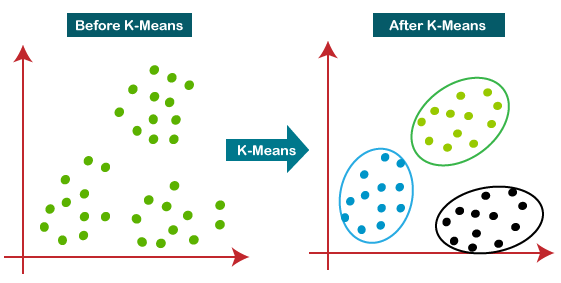
\includegraphics[width=0.7\textwidth]{images/kmeans.png}
    \caption{Set of data before and after the application of the K-Means algorithm}
    \label{fig:k_means}
\end{figure}


\subsection{Advantages and Limitations}
K-means is valued for its simplicity, efficiency, and scalability:
\begin{itemize}
    \item \textbf{Simplicity}: Easy to implement and interpret.
    \item \textbf{Efficiency}: Computationally efficient for moderate values of \( K \) and large datasets.
    \item \textbf{Versatility}: Applicable to a wide range of domains, including image compression and customer segmentation.
\end{itemize}


Despite its strengths, K-means has several limitations:
\begin{itemize}
    \item \textbf{Choice of \( K \)}: Requires prior knowledge of the number of clusters.
    \item \textbf{Initialization Sensitivity}: Poor initialization can lead to suboptimal clustering.
    \item \textbf{Cluster Shape Assumption}: Assumes clusters are spherical and of equal size, which may not hold for all datasets.
    \item \textbf{Outliers}: Sensitive to outliers, which can distort cluster centroids.
\end{itemize}

\subsection{Applications}

K-means clustering has numerous applications, including:
\begin{itemize}
    \item \textbf{Image Processing}: Color quantization and compression by reducing the number of colors in an image.
    \item \textbf{Market Segmentation}: Grouping customers based on purchasing behavior for targeted marketing.
    \item \textbf{Data Summarization}: Simplifying datasets by grouping similar data points.
    \item \textbf{Anomaly Detection}: Identifying outliers as data points that do not fit into any cluster well.
\end{itemize}

\subsection{Conclusion}

K-means clustering remains a foundational algorithm in machine learning due to its simplicity and effectiveness in solving clustering problems. While it has limitations, various extensions and initialization strategies, such as K-means++, have been developed to address these issues and improve the algorithm's robustness.


\section{Color Quantization}

Color quantization is a process used in image processing to reduce the number of distinct colors in an image while preserving its visual quality as much as possible. This is achieved by mapping the colors of the image to a smaller set of representative colors, known as a color palette. The result is a compressed image that retains its key visual features while using fewer colors.

\subsection{Purpose and Applications}

The main purpose of color quantization is to optimize image storage, processing, and transmission by reducing the complexity of the color information. It is widely used in several fields, including:

\begin{itemize}
    \item \textbf{Image Compression}: Reducing storage requirements for digital images by representing them with fewer colors.
    \item \textbf{Computer Graphics}: Rendering images efficiently on devices with limited color display capabilities.
    \item \textbf{Printing}: Mapping colors to a specific printer color gamut to ensure accurate reproduction.
    \item \textbf{Artistic Filters}: Creating stylized effects, such as cartoonization or posterization, by limiting the number of colors.
\end{itemize}

\subsection{Quantization Process}

The process of color quantization typically involves the following steps:

\begin{enumerate}
    \item \textbf{Color Space Selection}: Choose a color space (e.g., RGB, HSV, or CIE-Lab) for representing the image's pixel values. The choice of color space can influence the effectiveness of quantization, as some spaces better capture perceptual differences between colors.
    
    \item \textbf{Clustering of Colors}: Group similar colors into clusters. Each cluster represents a single color in the reduced palette. Clustering algorithms, such as K-means, are commonly used for this purpose. The goal is to minimize the perceptual difference between the original image and the quantized image.
    
    \item \textbf{Color Mapping}: Replace the original colors of the image with the nearest colors from the reduced palette. This step assigns each pixel in the image to the color of its cluster centroid.
\end{enumerate}

\begin{figure}[H]
    \centering
    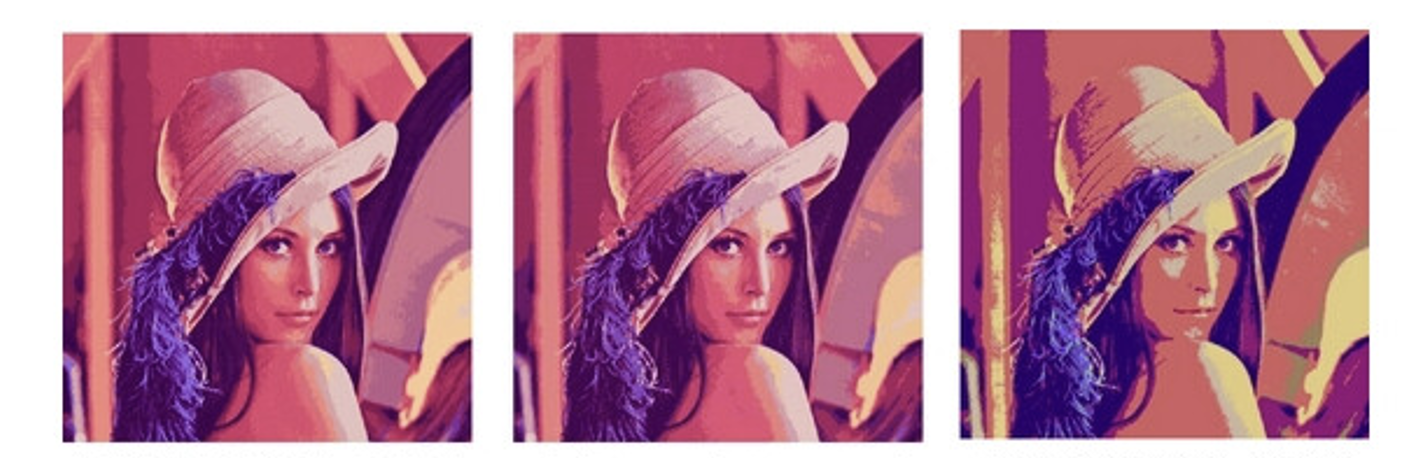
\includegraphics[width=0.7\textwidth]{images/color_quantization.png}
    \caption{Different color quantization algorithms applied to the same image}
    \label{fig:color_quantization}
\end{figure}

\subsection{Challenges in Color Quantization}

Color quantization is not without its challenges, which include:

\begin{itemize}
    \item \textbf{Perceptual Quality}: Reducing the number of colors can lead to visible artifacts or loss of detail, especially in images with subtle gradients.
    \item \textbf{Optimal Palette Selection}: Determining the optimal number and placement of colors in the palette is critical for balancing compression and visual fidelity.
    \item \textbf{Computational Cost}: Algorithms like K-means can be computationally expensive for high-resolution images, particularly with a large number of clusters.
    \item \textbf{Handling Outliers}: Outlier colors that do not belong to any major cluster can significantly affect the quality of the quantized image.
\end{itemize}


\subsection{Conclusion}

Color quantization is a crucial step in many image processing applications, balancing the trade-off between reducing storage requirements and maintaining visual quality. Techniques such as K-means clustering and median cut have been instrumental in achieving effective quantization, though challenges remain in optimizing perceptual quality and computational efficiency. In this work, color quantization plays a key role in achieving the desired cartoon-style effect by reducing the complexity of the image while preserving its essential features.


\chapter{Technologies}
\subsection{CUDA}

CUDA (Compute Unified Device Architecture) is a parallel computing platform and application programming interface (API) developed by NVIDIA. It enables developers to utilize the power of NVIDIA GPUs for general-purpose computing tasks. By leveraging CUDA, applications can perform computations faster by distributing tasks across thousands of GPU cores. It is widely used in fields such as scientific computing, machine learning, and real-time rendering.


\subsubsection{NVIDIA Nsight Compute}
NVIDIA Nsight Compute is a performance analysis tool designed for CUDA applications. It provides detailed metrics and insights into GPU kernel execution, enabling developers to identify bottlenecks and optimize their code. This tool is essential for understanding and improving the performance of GPU-accelerated applications.

\subsubsection{NVIDIA Nsight Systems}
NVIDIA Nsight Systems is a system-wide performance analysis tool that helps developers identify performance issues across the CPU and GPU. It provides a holistic view of application behavior, enabling optimization at both the system and application levels.

In the results section, we will analyze our findings using these tools to evaluate the performance of our CUDA-based implementations.

\subsection{OpenCV}

OpenCV (Open Source Computer Vision Library) is an open-source library designed for real-time computer vision and image processing tasks. It provides a wide range of tools and functions for image manipulation, feature extraction, object detection, and more. OpenCV is widely adopted in industries such as robotics, medical imaging, and autonomous vehicles due to its versatility and robust performance.

Some key features of OpenCV include:
\begin{itemize}
\item \textbf{Wide Functionality:} OpenCV supports tasks such as image filtering, geometric transformations, and object recognition.
\item \textbf{Cross-Platform Support:} OpenCV works on multiple platforms, including Windows, Linux, macOS, and Android.
\item \textbf{Hardware Acceleration:} OpenCV integrates with CUDA and OpenCL to accelerate processing on compatible hardware.
\end{itemize}

OpenCV is written in C++ but provides bindings for Python, Java, and other languages, making it accessible to a wide range of developers. With its comprehensive functionality and active community, OpenCV remains a cornerstone of computer vision development.


\chapter{Technical implementation}
In this chapter, we present an overview of our work on implementing k-means clustering algorithms for image processing. Two distinct approaches have been developed, each tailored to different computational paradigms and performance goals:

\begin{itemize}
\item \textbf{Sequential Algorithm:} A straightforward implementation in C++ that processes the input image using the k-means clustering technique. This version, while simple and easy to understand, is optimized for single-threaded execution and serves as a baseline for performance comparisons.
\item \textbf{Parallel Algorithm with CUDA:} A high-performance version of the k-means algorithm designed to utilize NVIDIA GPUs. This approach leverages CUDA to perform computations in parallel across thousands of GPU cores, providing significant speedups for large-scale image data.
\end{itemize}

These implementations highlight the trade-offs between simplicity and performance, and they serve as a foundation for evaluating the impact of parallelization on clustering algorithms. The following sections will delve into the specifics of each implementation, detailing their design, execution, and performance considerations.

\section{Sequential cartoonizer}
We will now break down and analyze different parts of the code, explaining how each segment works and contributes to the overall functionality of the cartoonizer.

\subsection{Euclidean Distance Function}
This function computes the Euclidean distance between two colors, which is essential for finding the nearest cluster centroid during the K-means algorithm.

\begin{lstlisting}[language=C++]
// Compute the Euclidean distance between two colors
float euclidean_distance(const Color& a, const Color& b) {
    return std::sqrt((a.r - b.r) * (a.r - b.r) + (a.g - b.g) * (a.g - b.g) + (a.b - b.b) * (a.b - b.b));
}
\end{lstlisting}

\textbf{Explanation:}
This function calculates the squared differences in the RGB values between two colors and returns the square root of the sum of those squared differences. This distance metric is used to compare how close two colors are in RGB space.

\subsection{Update Centroids Function}
After assigning each pixel to the nearest centroid, the centroids need to be updated by averaging the pixel colors assigned to each cluster.

\begin{lstlisting}[language=C++]
// Update centroids based on pixel assignments
void update_centroids(const std::vector<Color>& pixels, const std::vector<int>& assignments, std::vector<Color>& centroids, int k) {
    std::vector<int> cluster_sizes(k, 0);
    std::vector<Color> new_centroids(k, {0.0f, 0.0f, 0.0f});

    for (size_t i = 0; i < pixels.size(); i++) {
        int cluster_idx = assignments[i];
        new_centroids[cluster_idx].r += pixels[i].r;
        new_centroids[cluster_idx].g += pixels[i].g;
        new_centroids[cluster_idx].b += pixels[i].b;
        cluster_sizes[cluster_idx]++;
    }

    for (int i = 0; i < k; i++) {
        if (cluster_sizes[i] > 0) {
            new_centroids[i].r /= cluster_sizes[i];
            new_centroids[i].g /= cluster_sizes[i];
            new_centroids[i].b /= cluster_sizes[i];
        }
    }

    centroids = new_centroids;
}
\end{lstlisting}

\textbf{Explanation:}
This function iterates over each pixel and updates the centroids by averaging the colors of all pixels assigned to each cluster. It ensures that the new centroids represent the average color of each cluster, which will be used in the next iteration.

\subsection{K-means Function}
The main function implementing the K-means algorithm for color quantization. It converts the image to a set of color values, applies the K-means clustering algorithm, and then generates the output image with reduced colors.

\begin{lstlisting}[language=C++]
// K-means algorithm for color quantization
void kmeans_cpu(const cv::Mat& image, int k, int max_iter, cv::Mat& output_image,int seed) {
    int width = image.cols;
    int height = image.rows;
    int num_pixels = width * height;

    // Convert image to a vector of Color structs
    std::vector<Color> pixels(num_pixels);
    for (int i = 0; i < height; i++) {
        for (int j = 0; j < width; j++) {
            cv::Vec3b color = image.at<cv::Vec3b>(i, j);
            pixels[i * width + j] = { color[2] / 255.0f, color[1] / 255.0f, color[0] / 255.0f };
        }
    }

    srand(seed);

    // Randomly initialize centroids
    std::vector<Color> centroids(k);
    for (int i = 0; i < k; i++) {
        centroids[i] = { float(rand()) / RAND_MAX, float(rand()) / RAND_MAX, float(rand()) / RAND_MAX };
    }

    std::vector<int> assignments(num_pixels, 0);
    for (int iter = 0; iter < max_iter; iter++) {
        // Step 1: Assign each pixel to the closest centroid
        for (int i = 0; i < num_pixels; i++) {
            float min_dist = std::numeric_limits<float>::max();
            for (int j = 0; j < k; j++) {
                float dist = euclidean_distance(pixels[i], centroids[j]);
                if (dist < min_dist) {
                    min_dist = dist;
                    assignments[i] = j;
                }
            }
        }

        // Step 2: Update centroids based on the pixel assignments
        update_centroids(pixels, assignments, centroids, k);
    }

    // Step 3: Create the output image
    output_image = image.clone();
    for (int i = 0; i < height; i++) {
        for (int j = 0; j < width; j++) {
            int cluster_idx = assignments[i * width + j];
            cv::Vec3b new_color(
                static_cast<unsigned char>(centroids[cluster_idx].b * 255),
                static_cast<unsigned char>(centroids[cluster_idx].g * 255),
                static_cast<unsigned char>(centroids[cluster_idx].r * 255)
            );
            output_image.at<cv::Vec3b>(i, j) = new_color;
        }
    }
}
\end{lstlisting}

\textbf{Explanation:}
- The function first converts the input image into a vector of `Color` structs. Each pixel’s RGB values are normalized between 0 and 1.
- It randomly initializes the centroids, assigns each pixel to the nearest centroid, and updates the centroids in each iteration.
- After \( \text{max\_iter} \) iterations, the final output image is generated where each pixel is replaced by the corresponding centroid color.

\subsection{Main Function}
The main driver code calls the functions, loads the image, applies K-means, and saves the output image.

\begin{lstlisting}[language=C++]
int main(int argc, char* argv[]) {
    int clusters = DEFAULT_CLUSTERS;
    int iterations = DEFAULT_ITERATIONS;
    int seed = DEFAULT_SEED;
    int threads_per_block = DEFAULT_THREADS;
    std::string input_image_path = "images/image.jpg";
    std::string output_image_path = "images/cartoon_cpu.jpg";

    arg_parser(argc, argv, clusters, iterations, seed, threads_per_block, input_image_path, output_image_path);

    // Load the image
    cv::Mat image = cv::imread(input_image_path);
    if (image.empty()) {
        std::cerr << "Error loading image!" << std::endl;
        return -1;
    }

    cv::Mat output_image;
    kmeans_cpu(image, clusters, iterations, output_image, seed);

    // Save the output
    cv::imwrite(output_image_path, output_image);
    std::cout << "CPU output saved!" << std::endl;
    return 0;
}
\end{lstlisting}

\textbf{Explanation:}
The main function reads the input image, applies the K-means algorithm, and saves the result as the output image.

\subsection{Conclusion}
The K-means algorithm used in this code provides an effective way to reduce the color complexity of an image, giving it a cartoon-like appearance. By analyzing and applying clustering to pixel colors, the image becomes more abstract and simplified, which enhances the cartoon effect.



\section{Parallel cartoonizer}
\chapter{Results}

We present the results of our performance evaluation. To assess the efficiency and improvements brought by the parallel CUDA implementation, we tested the algorithm on three different machines, each with distinct hardware specifications. 

For each machine, we conducted six tests with varying configurations, including different image sizes, numbers of clusters, and thread configurations. This allowed us to analyze how the algorithm scales with different hardware and computational loads.

The three tested machines are as follows:

\begin{itemize}
    \item \textbf{Machine 1:} Equipped with an \textbf{NVIDIA GeForce GTX 1660} GPU (Turing architecture, 1536 CUDA cores, 6GB GDDR5 VRAM) and an \textbf{Intel Core i5-9600K} CPU (6 cores, 6 threads, 2.2GHz). This represents a mid-range consumer-grade system.
    
    \item \textbf{Machine 2:} Featuring an \textbf{NVIDIA GeForce RTX 4060} GPU (Ada Lovelace architecture, 3072 CUDA cores, 8GB GDDR6 VRAM) and an \textbf{AMD Ryzen 5 3600} CPU (6 cores, 12 threads, 2.2GHz). This machine is the most powerful among the tested ones, providing insights into high-performance configurations.

    \item \textbf{Machine 3:} A workstation-class system with an \textbf{NVIDIA Quadro K5000} GPU (Kepler architecture, 1536 CUDA cores, 4GB GDDR5 VRAM) and an \textbf{Intel Core i7} CPU (4 cores, 2.8GHz). This represents an older generation of hardware, providing a benchmark for performance on legacy systems.
\end{itemize}

The following subsections present and analyze the execution times and speedups achieved under different configurations.

\section{How the results are collected}
Each session folder has a README.md file that contains the main results of the session such as execution time, speedup, output image yielded by the program, and so on.

An advanced insights are contained in the binary files named report.ncu-rep, theese files provid detailed information about the execution of the CUDA kernels, in this way we were able to analyze common issues about CUDA kernels, such as bottleneck problem.

The report.ncu-rep files were generated using NVIDIA Nsight Compute, so to read it you have to install this tool, then you have to launch the follow command on your terminal:

\begin{lstlisting}[basicstyle=\ttfamily\footnotesize\color{white}, backgroundcolor=\color{black}, keywordstyle=\color{white}, stringstyle=\color{white}, identifierstyle=\color{white}]
    ncu-ui "report.ncu-rep"
\end{lstlisting}





For the GPUs that has a compute capability lower than 7.0 we weren't able to use Nsight Compute, for this reason we have used nvprof tool to collect insights on theese generation of GPUs; nvprof profiling are stored in the files called output.nvprof.
The results are visualizable only using NVIDIA Visual Profiler. Anyway a profiler.output.txt file has been generated for summary insights.



\section{Test 1}
\begin{figure}[H]
    \centering
    \begin{minipage}[b]{0.45\textwidth}
        \centering
        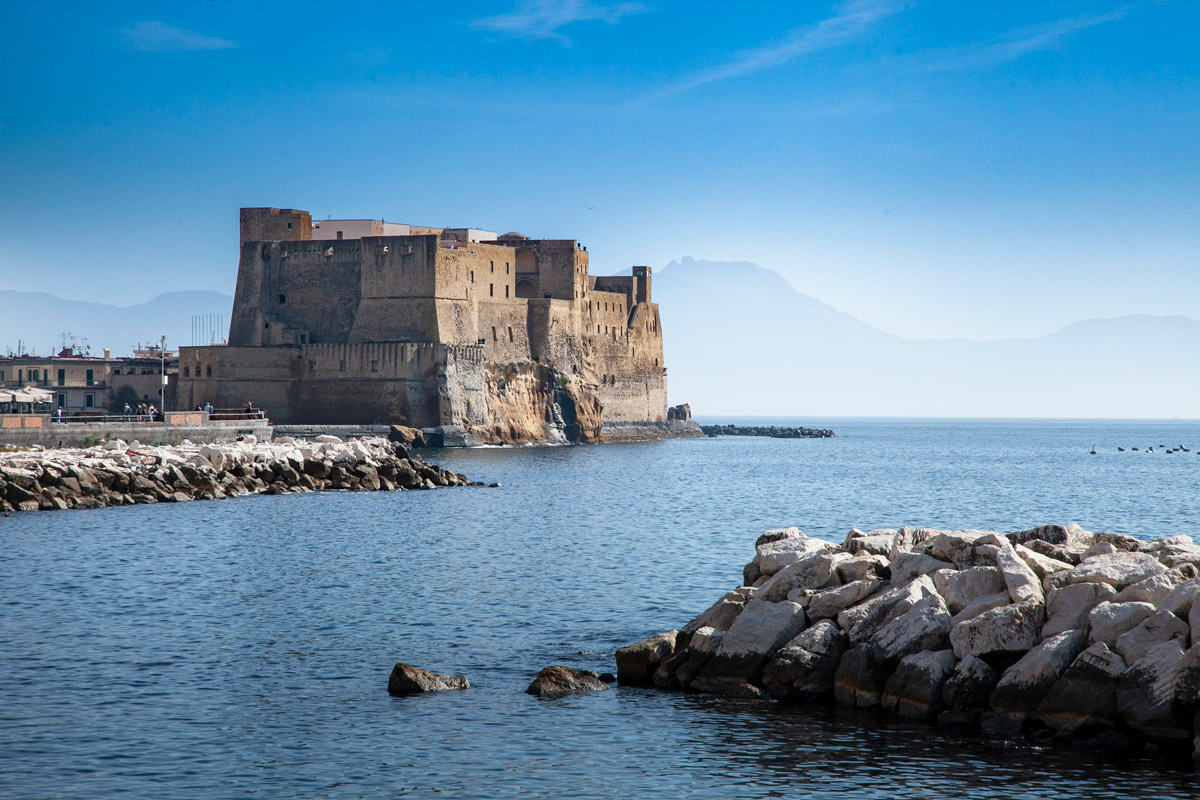
\includegraphics[width=\textwidth]{images/input_image_t1.jpg}
        \caption{(a) Input image.}
        \label{fig:test_1_input}
    \end{minipage}
    \hfill
    \begin{minipage}[b]{0.45\textwidth}
        \centering
        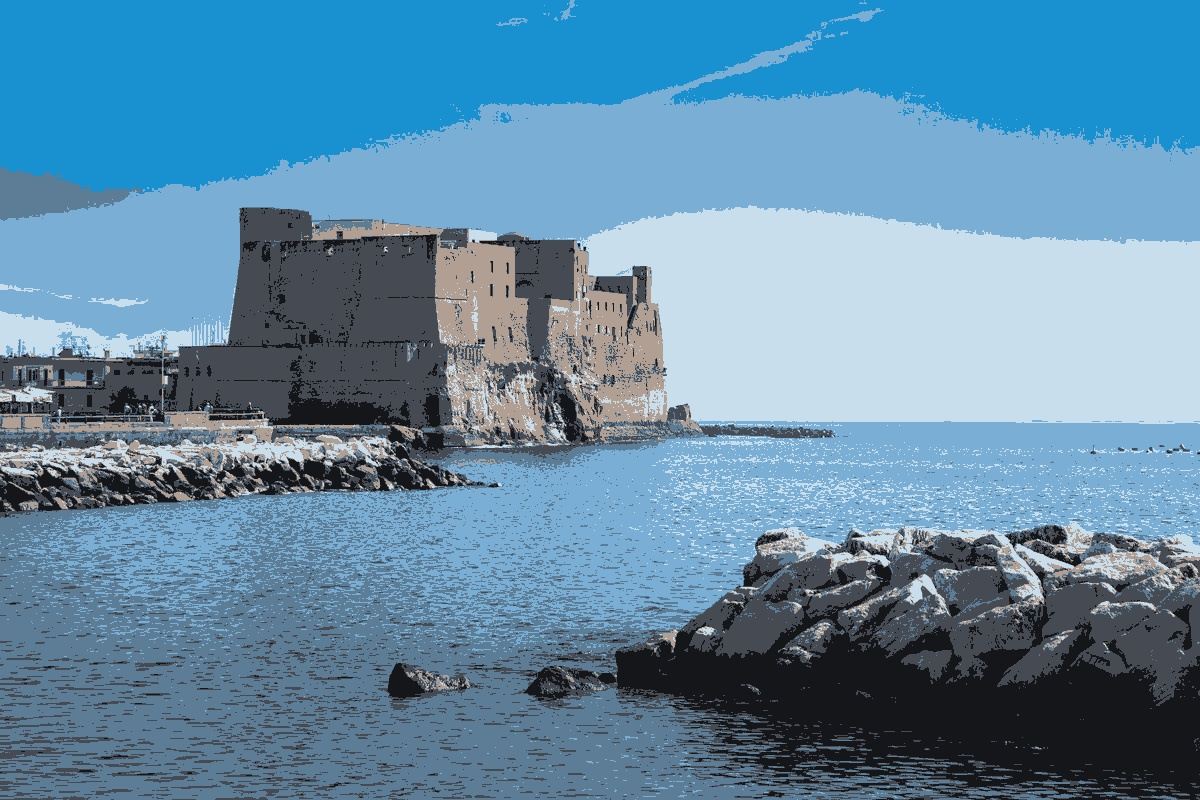
\includegraphics[width=\textwidth]{images/output_image_t1.jpg}
        \caption{(b) Output image.}
        \label{fig:test_1_output}
    \end{minipage}
    \end{figure}
    
\begin{table}[H]
    \centering
    \begin{tabular}{|l|l|}
    \hline
    \textbf{Input Info} & \textbf{Value} \\ \hline
    Session ID          & 0              \\ \hline
    Image width         & 1200px         \\ \hline
    Image height        & 800px          \\ \hline
    Image channels      & RGB (3 channels) \\ \hline
    \#Clusters          & 7              \\ \hline
    \#Iterations        & 50             \\ \hline
    \#Threads           & 256            \\ \hline
    Random seed         & 200            \\ \hline
    \end{tabular}
    \caption{Session information}
    \label{table:session_information_test1}
    \end{table}
    
\subsection{GeForce 1660}

    \begin{table}[H]
        \centering
        \begin{tabular}{|l|l|}
        \hline
        \textbf{Metric}                     & \textbf{Value}                \\ \hline
        Execution time (Parallel version)   & ~569ms (0.59s)                \\ \hline
        Execution time (Sequential version) & ~5034ms (5s)                  \\ \hline
        Delta time                          & +4438ms (+4.4s)               \\ \hline
        Speedup                             & 8.84                          \\ \hline
        \end{tabular}
        \caption{Performance Metrics on \textbf{Machine 1}}
        \label{table:performance_metrics_test1_machine1}
        \end{table}
        

\subsection{Geforce 4060}
\begin{table}[H]
    \centering
    \begin{tabular}{|l|l|}
    \hline
    \textbf{Metric}                         & \textbf{Value}                       \\ \hline
    Execution time (Parallel version)       & ~450ms (0.45s)                        \\ \hline
    Execution time (Sequential version)     & ~4000ms (4s)                          \\ \hline
    Delta time                               & +3550ms (+3.5s)                       \\ \hline
    Speedup                                  & 8.8                                   \\ \hline
    \end{tabular}
    \caption{Performance Metrics on \textbf{Machine 2}}
    \label{tab:performance_metrics_test1_machine2}
    \end{table}
    
\subsection{Quadro K5000}
\begin{table}[H]
    \centering
    \begin{tabular}{|l|l|}
    \hline
    \textbf{Metric}                         & \textbf{Value}                       \\ \hline
    Execution time (Parallel version)       & ~1451ms (1.45s)                       \\ \hline
    Execution time (Sequential version)     & ~11630ms (11.63s)                     \\ \hline
    Delta time                               & +10179ms (+10.17s)                    \\ \hline
    Speedup                                  & 8                                     \\ \hline
    \end{tabular}
    \caption{Performance Metrics on \textbf{Machine 3}}
    \label{tab:performance_metrics_test1_machine3}
    \end{table}
    
\subsection{Conclusion}
In conclusion, the results from the three different machines show varied performance metrics with respect to execution time, speedup, and efficiency. As expected, the parallel version of the task consistently outperforms the sequential version in all cases, with the speedup ranging from 8x to 9x across the tested machines. 

The GeForce 1660 machine performed well with a speedup of 8.84, while the Geforce 4060 machine showed a slightly lower speedup of 8.8. Interestingly, the Quadro K5000 machine, while having a significant sequential execution time, achieved a speedup of 8. This shows the importance of parallelization in reducing the processing time on different hardware configurations. Further tests with different image sizes or more threads could provide even more insights into how well these machines scale with different workloads.

The parallel implementation not only demonstrated a clear advantage in terms of speedup but also allowed the machines to efficiently handle larger input sizes, further highlighting the importance of parallel computation in modern hardware environments.

\section{Test 2}
\begin{figure}[H]
    \centering
    \begin{minipage}[b]{0.45\textwidth}
        \centering
        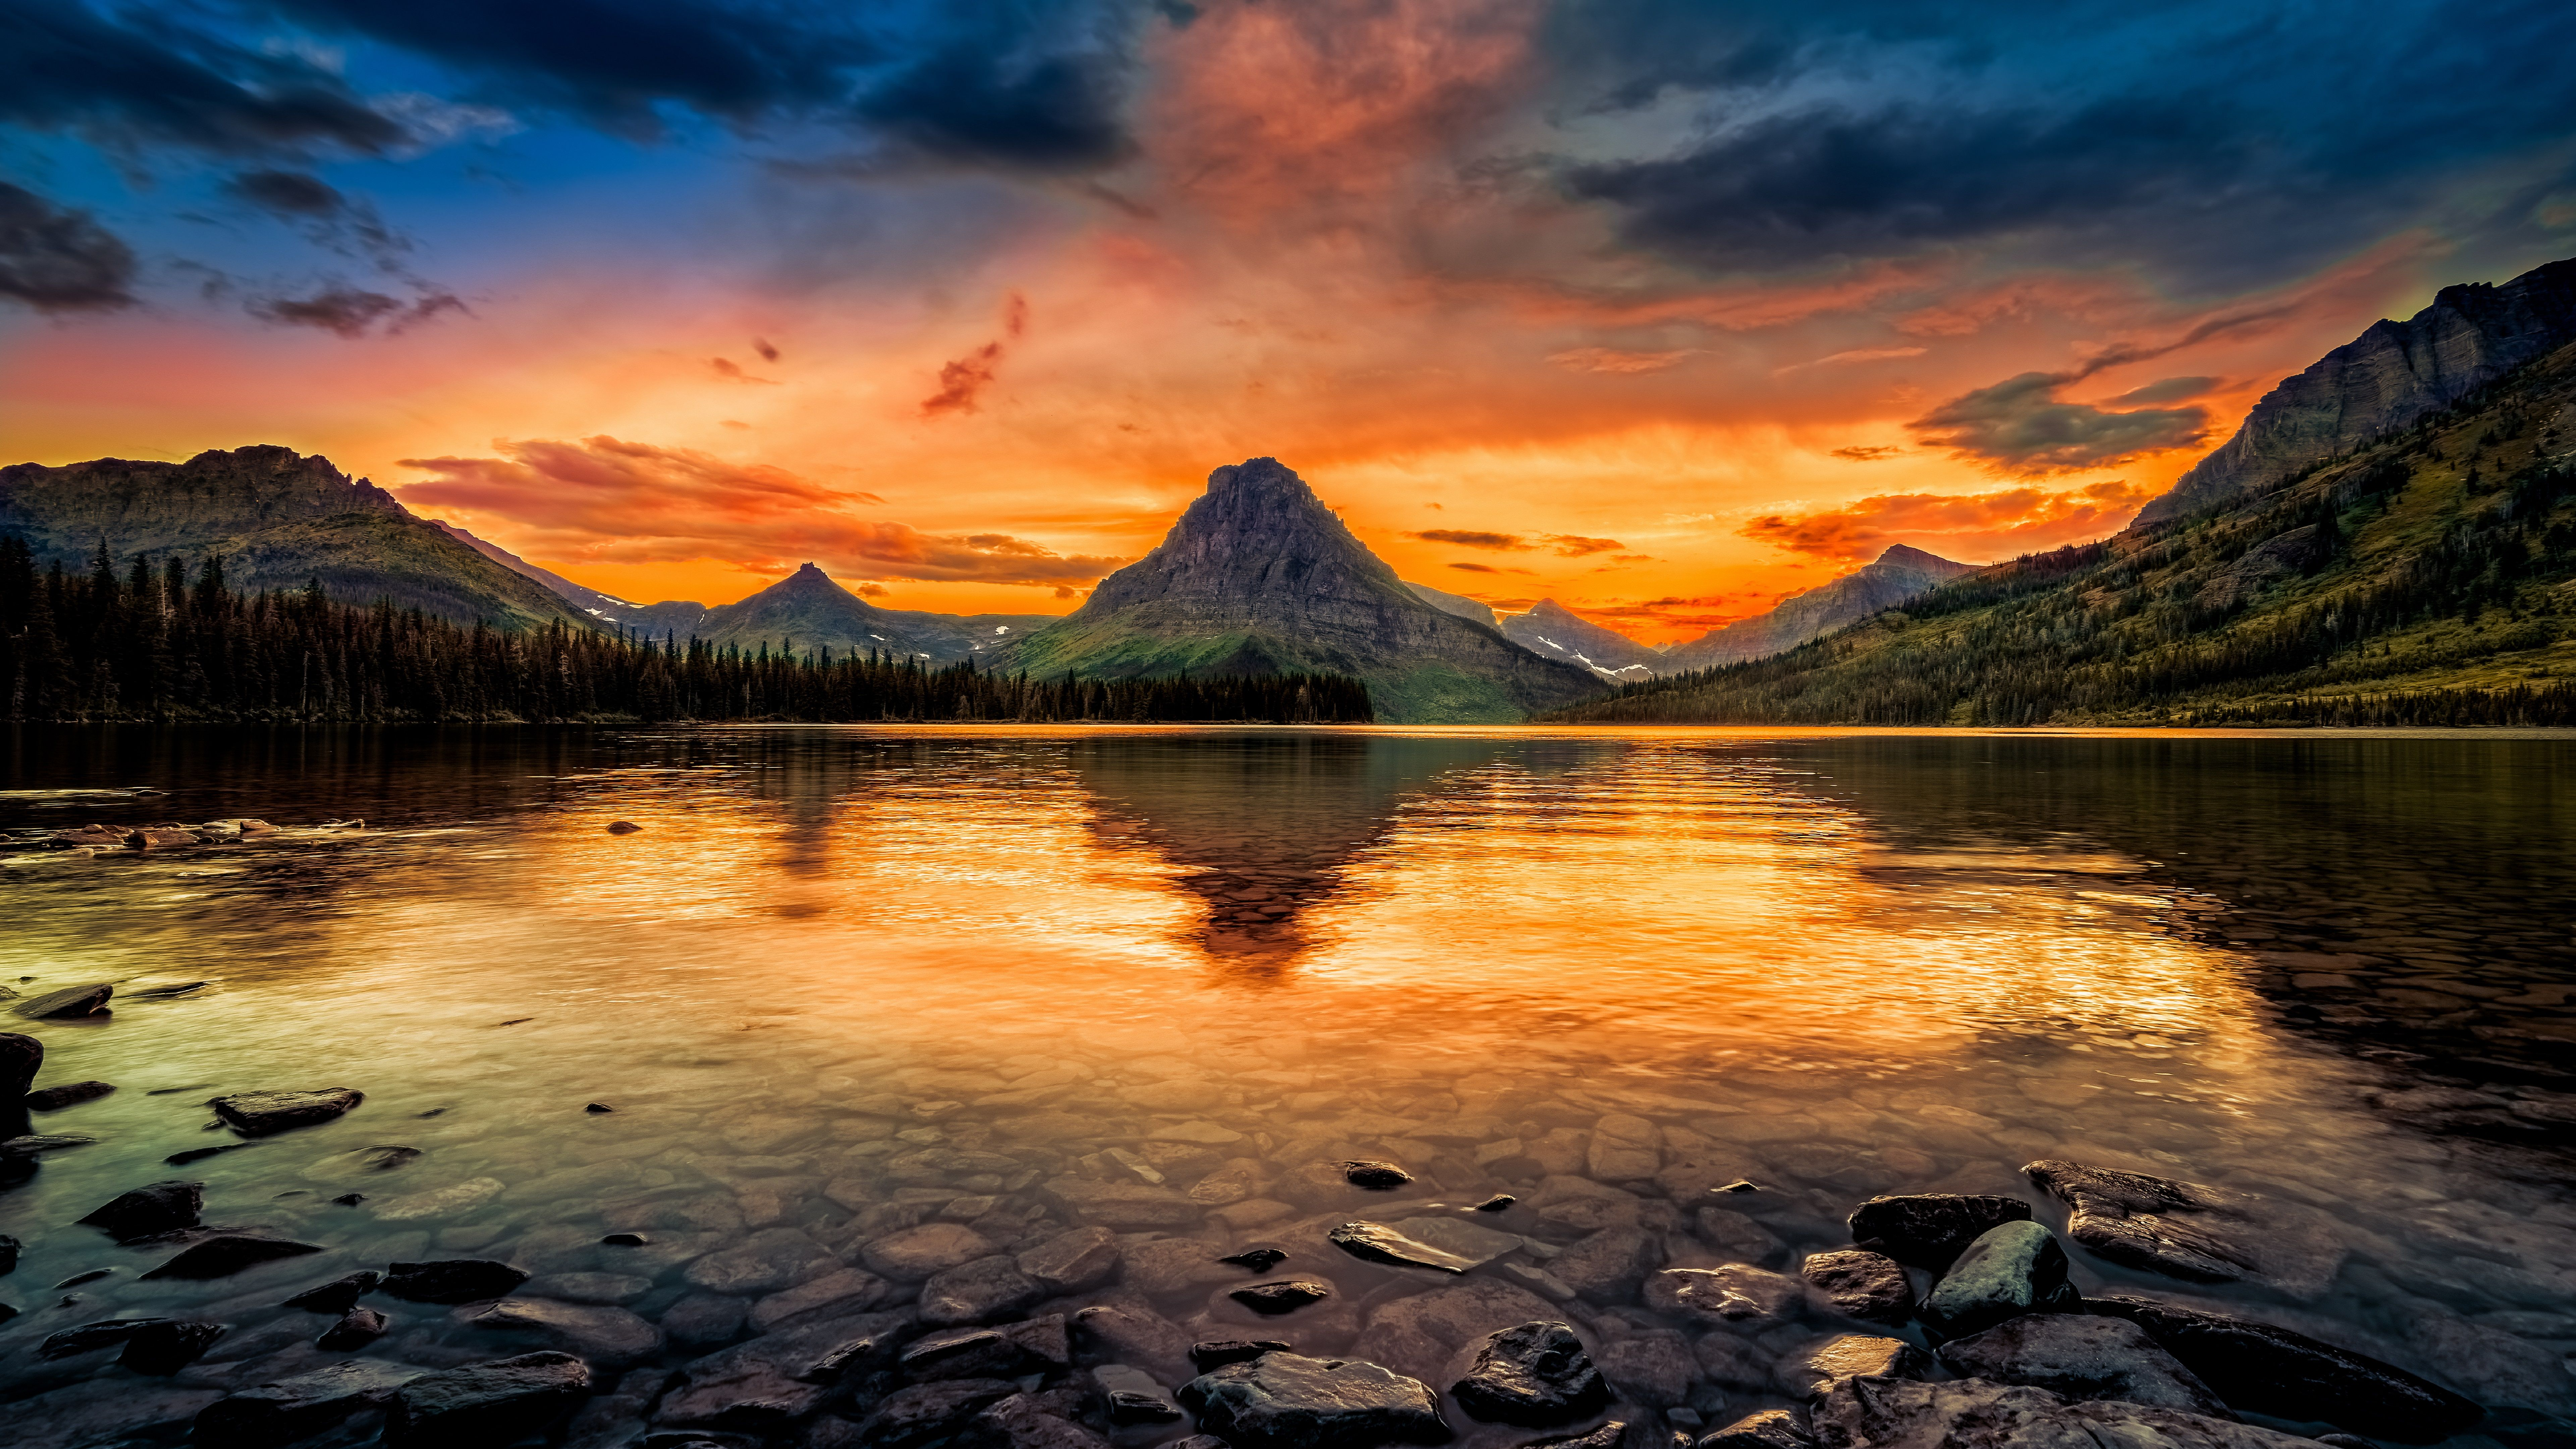
\includegraphics[width=\textwidth]{images/input_image_t2.jpg}
        \caption{(a) Input image.}
        \label{fig:test_2_input}
    \end{minipage}
    \hfill
    \begin{minipage}[b]{0.45\textwidth}
        \centering
        \includegraphics[width=\textwidth]{images/output_image_t2.jpg}
        \caption{(b) Output image.}
        \label{fig:test_2_output}
    \end{minipage}
    \end{figure}

    \begin{table}[H]
        \centering
        \begin{tabular}{|l|l|}
        \hline
        \textbf{Input Info}                    & \textbf{Value}                       \\ \hline
        Session ID                             & 1                                     \\ \hline
        Image width                            & 7680px                                \\ \hline
        Image height                           & 4320px                                \\ \hline
        Image channels                         & RGB (3 channels)                      \\ \hline
        \#Clusters                             & 7                                     \\ \hline
        \#Iterations                           & 50                                    \\ \hline
        \#Threads                              & 256                                   \\ \hline
        Random seed                            & 200                                   \\ \hline
        \end{tabular}
        \caption{Session information}
        \label{tab:session_information_test2}
        \end{table}
        

        \subsection{GeForce 1660}

        \begin{table}[H]
            \centering
            \begin{tabular}{|l|l|}
            \hline
            \textbf{Metric}                         & \textbf{Value}                       \\ \hline
            Execution time (Parallel version)       & ~19885ms (19.88s)                     \\ \hline
            Execution time (Sequential version)     & ~163264ms (2.7 minutes)               \\ \hline
            Delta time                               & +143379ms (+2.38 minutes)             \\ \hline
            Speedup                                  & 8.21                                   \\ \hline
            \end{tabular}
            \caption{Performance Metrics on \textbf{Machine 1}}
            \label{table:performance_metrics_test2_machine1}
        \end{table}
        
        
        \subsection{Geforce 4060}
        
        \begin{table}[H]
            \centering
            \begin{tabular}{|l|l|}
            \hline
            \textbf{Metric}                         & \textbf{Value}                       \\ \hline
            Execution time (Parallel version)       & ~19000ms (19s)                        \\ \hline
            Execution time (Sequential version)     & ~150000ms (2.5 minutes)               \\ \hline
            Delta time                               & +148000ms (+1.40 minutes)            \\ \hline
            Speedup                                  & 78.94                                  \\ \hline
            \end{tabular}
            \caption{Performance Metrics on \textbf{Machine 2}}
            \label{table:performance_metrics_test2_machine2}
        \end{table}
        
        
        \subsection{Quadro K5000}
        
        \begin{table}[H]
            \centering
            \begin{tabular}{|l|l|}
            \hline
            \textbf{Metric}                         & \textbf{Value}                       \\ \hline
            Execution time (Parallel version)       & ~50608ms (50.60s)                     \\ \hline
            Execution time (Sequential version)     & ~398440ms (6.64 minutes)              \\ \hline
            Delta time                               & +347832ms (+5.79 minutes)            \\ \hline
            Speedup                                  & 7.87                                   \\ \hline
            \end{tabular}
            \caption{Performance Metrics on \textbf{Machine 3}}
            \label{table:performance_metrics_test2_machine3}
        \end{table}

\subsection{Conclusion}
In Test 2, we observed significant improvements in performance across all three machines tested, particularly in the parallel execution versions. The GeForce 1660 achieved a speedup of 8.21, with a substantial reduction in execution time compared to the sequential version. The Geforce 4060 showed an even more impressive performance with a speedup of 78.94, demonstrating its strong ability to handle parallel tasks efficiently. Meanwhile, the Quadro K5000, while lagging behind in speedup at 7.87, still exhibited a noteworthy improvement over the sequential execution.

These results emphasize the importance of parallel processing, especially when dealing with larger image sizes and complex computations. The differences in performance between the machines highlight the varying capabilities of the hardware, with newer or more powerful GPUs (like the Geforce 4060) offering a much greater reduction in processing time compared to older models. Overall, the parallel implementation proved to be highly effective, achieving notable speedups in all cases, and further optimization could push these numbers even higher.

\section{Test 3}
\begin{figure}[H]
    \centering
    \begin{minipage}[b]{0.45\textwidth}
        \centering
        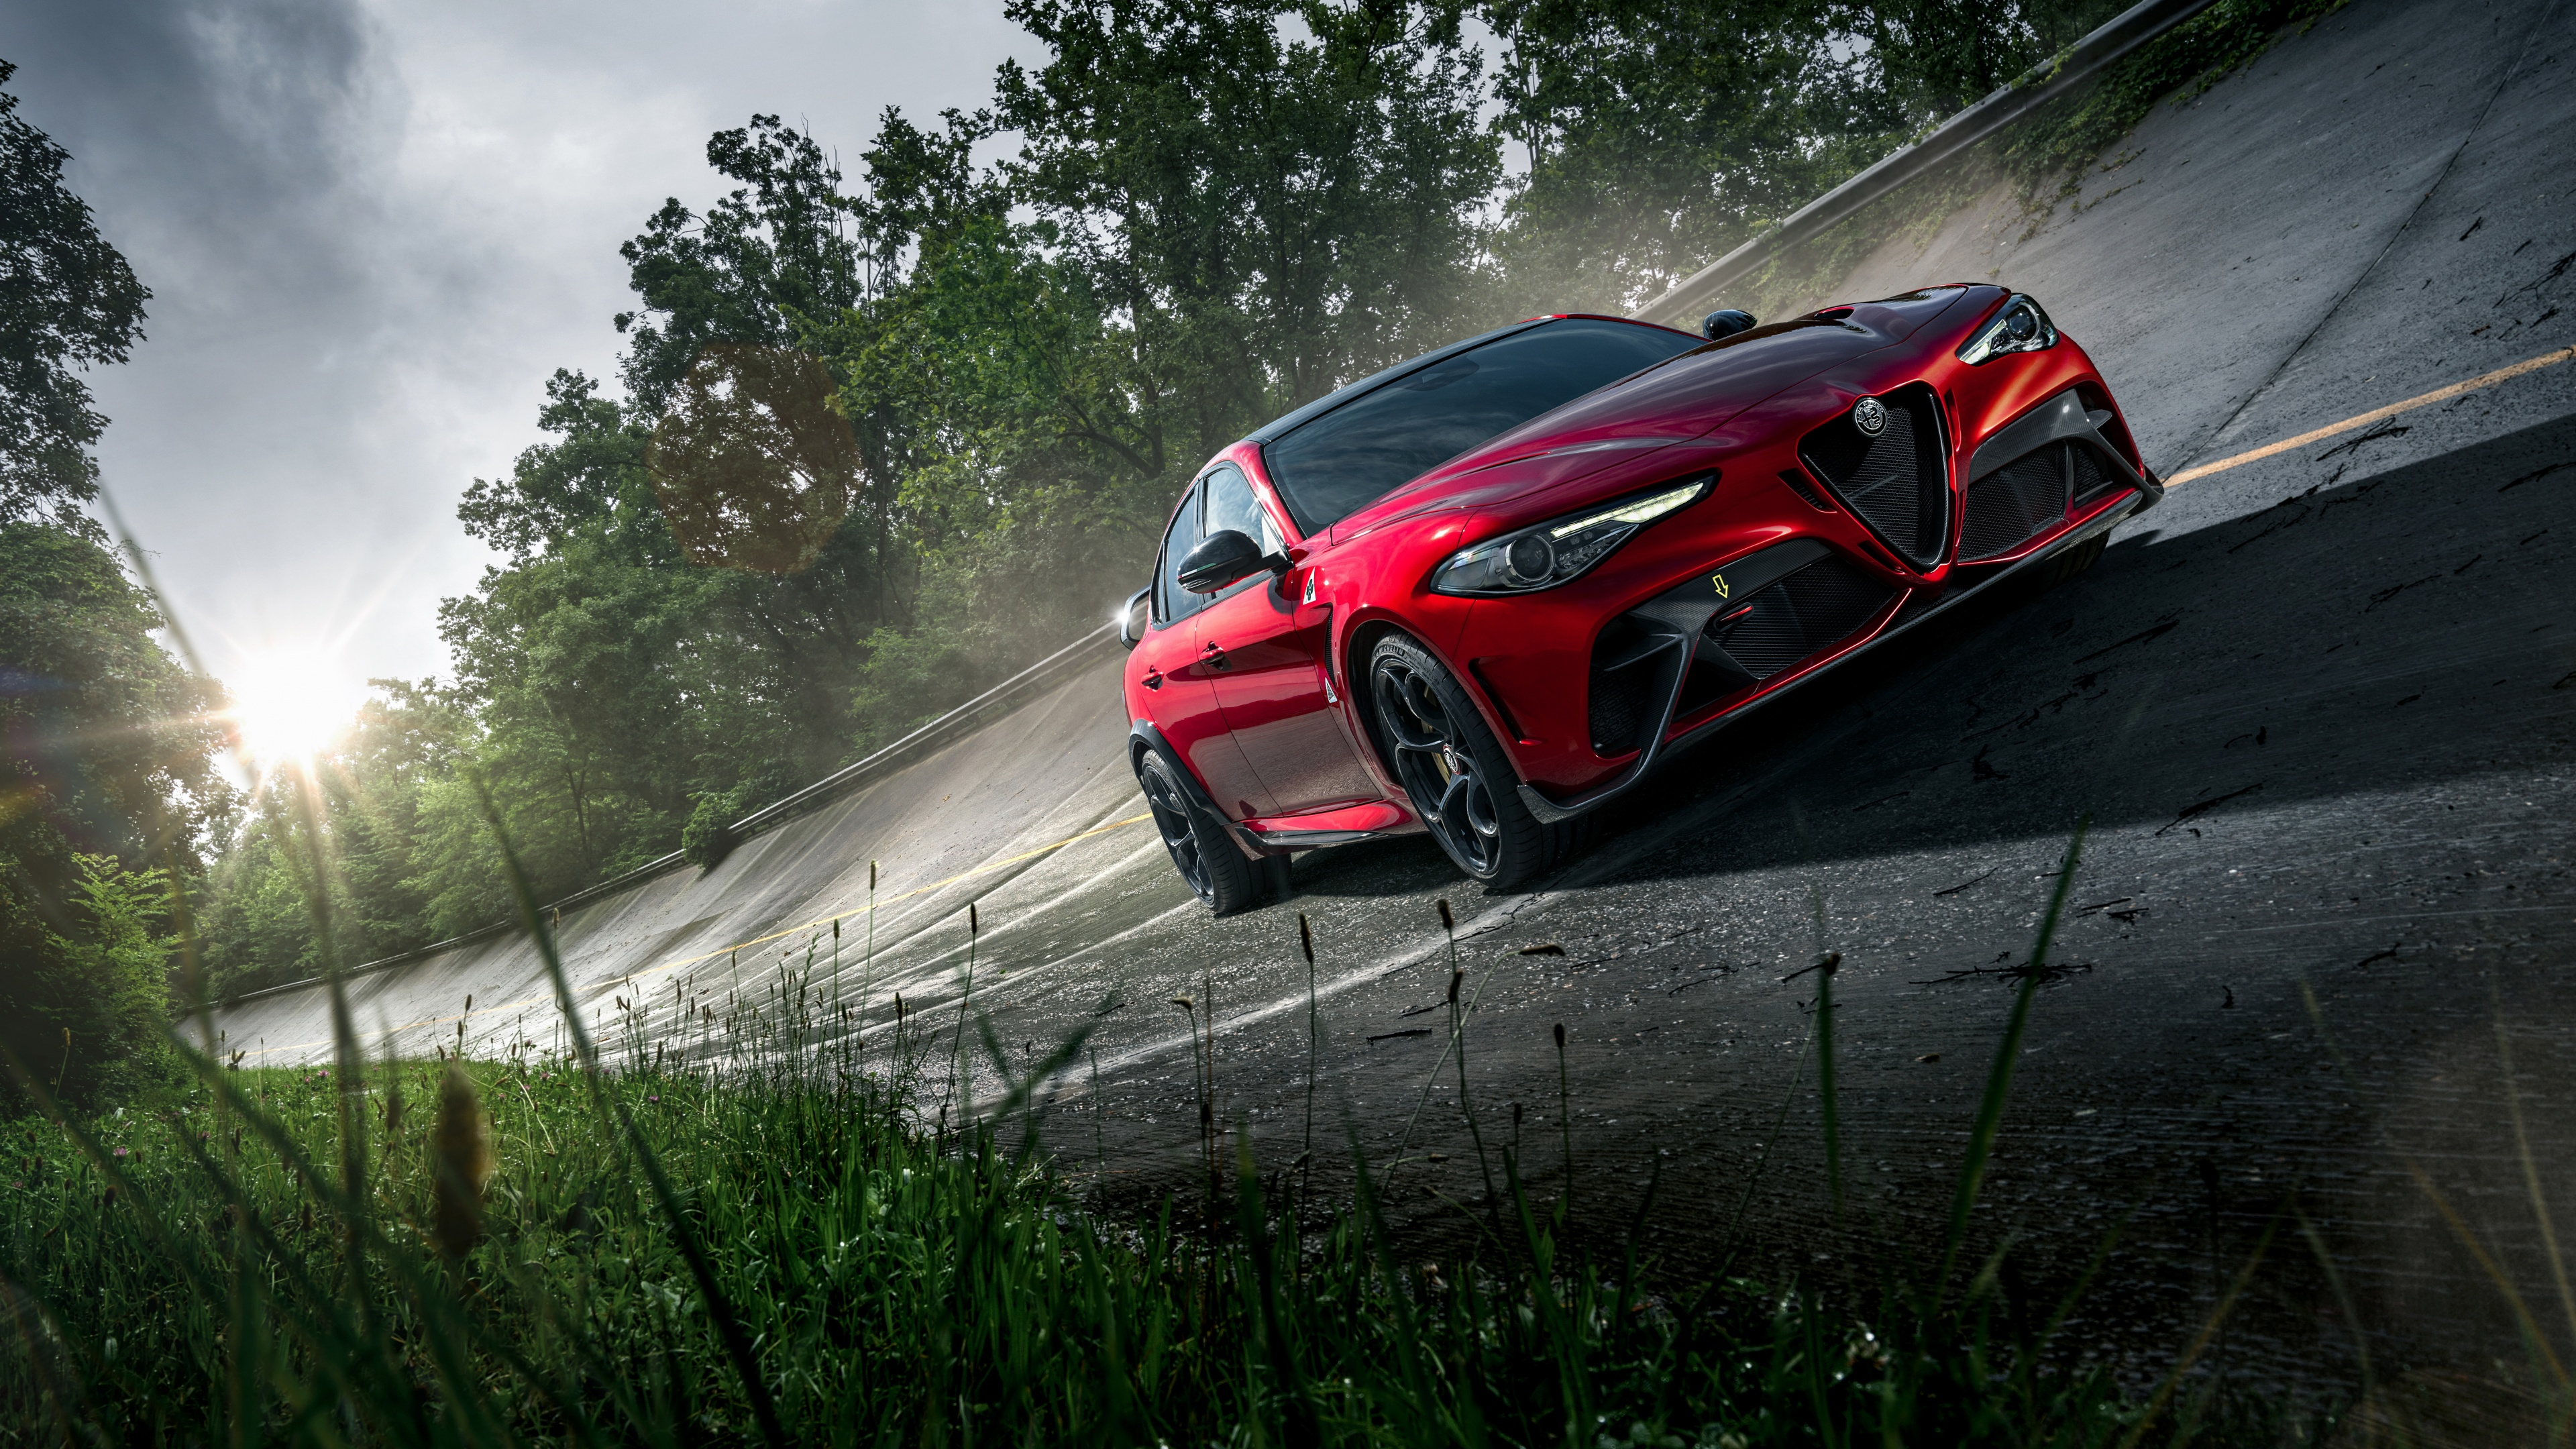
\includegraphics[width=\textwidth]{images/input_image_t3.jpg}
        \caption{(a) Input image.}
        \label{fig:test_3_input}
    \end{minipage}
    \hfill
    \begin{minipage}[b]{0.45\textwidth}
        \centering
        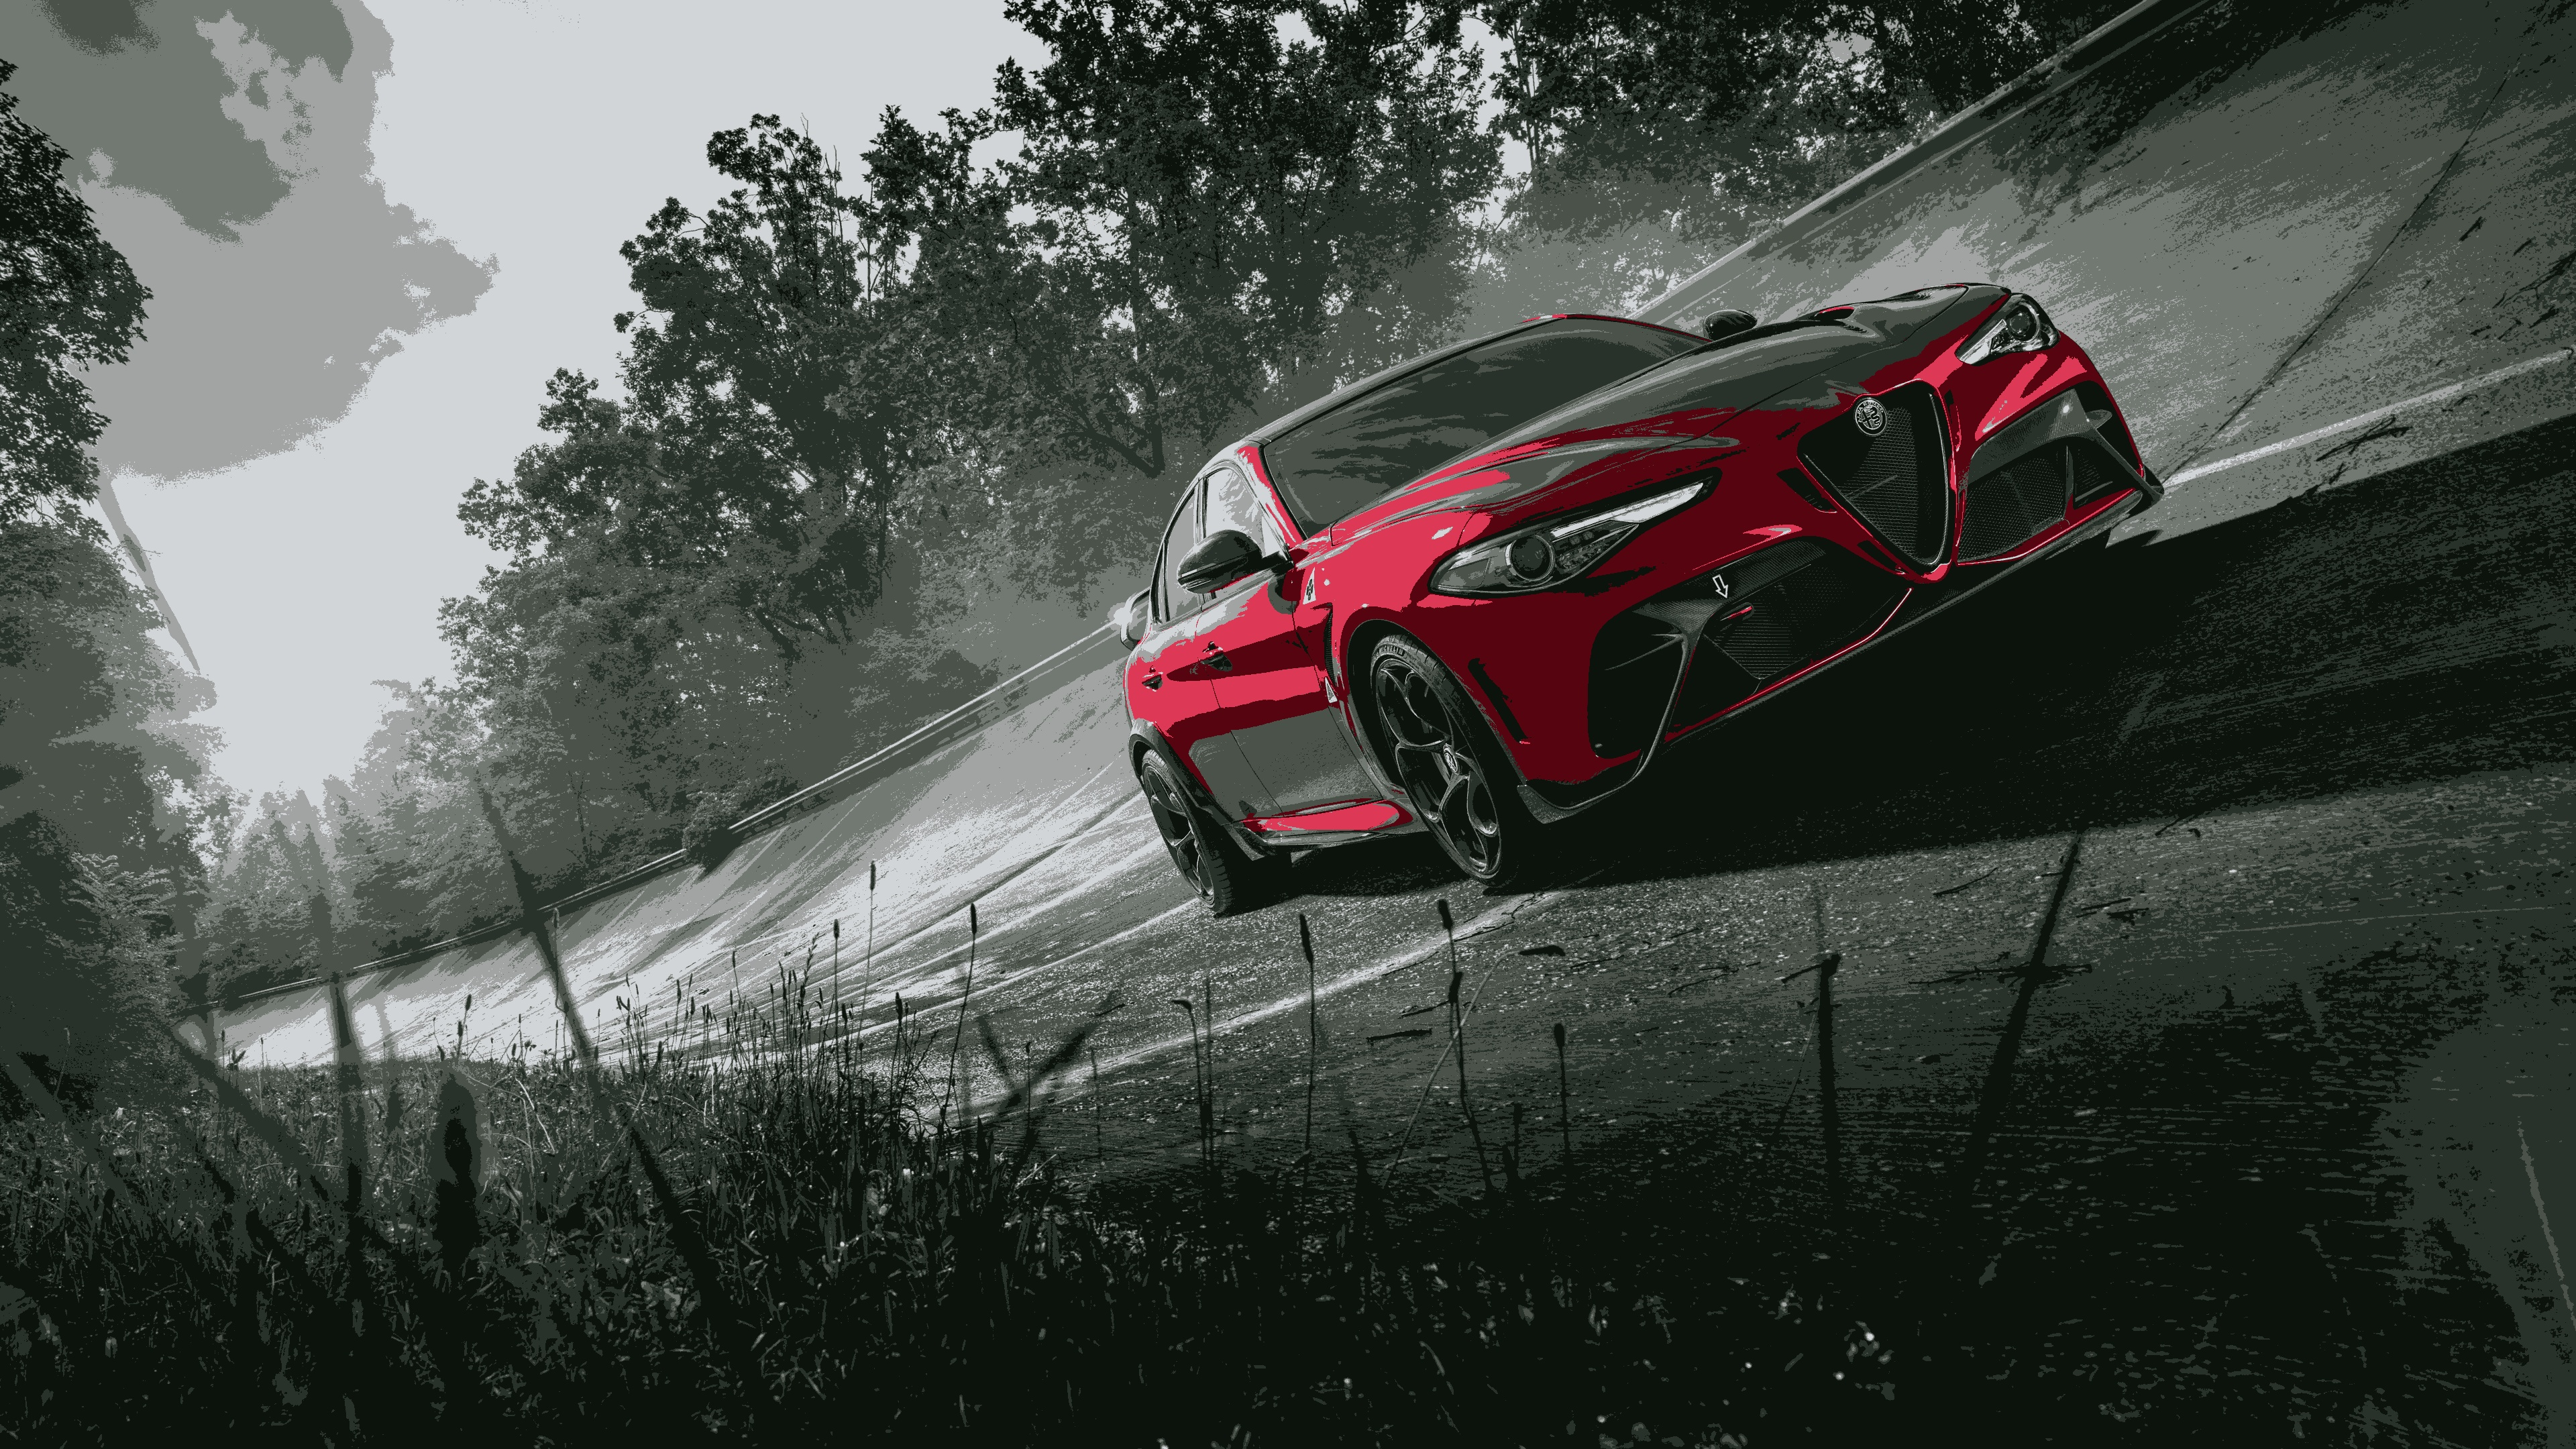
\includegraphics[width=\textwidth]{images/output_image_t3.jpg}
        \caption{(b) Output image.}
        \label{fig:test_3_output}
    \end{minipage}
    \end{figure}

    \begin{table}[H]
        \centering
        \begin{tabular}{|l|l|}
        \hline
        \textbf{Input Info}                    & \textbf{Value}                       \\ \hline
        Session ID                             & 2                                     \\ \hline
        Image width                            & 3840px                                \\ \hline
        Image height                           & 2160px                                \\ \hline
        Image channels                         & RGB (3 channels)                      \\ \hline
        \#Clusters                             & 8                                     \\ \hline
        \#Iterations                           & 50                                    \\ \hline
        \#Threads                              & 128                                   \\ \hline
        Random seed                            & 200                                   \\ \hline
        \end{tabular}
        \caption{Session information}
        \label{tab:session_information_test3}
        \end{table}
        
        \subsection{GeForce 1660}

        \begin{table}[H]
            \centering
            \begin{tabular}{|l|l|}
            \hline
            \textbf{Metric}                         & \textbf{Value}                       \\ \hline
            Execution time (Parallel version)       & ~4397ms (4.39s)                       \\ \hline
            Execution time (Sequential version)     & ~41379ms (41.37s)                     \\ \hline
            Delta time                               & +36982ms (+36.98s)                    \\ \hline
            Speedup                                  & 9.4                                    \\ \hline
            \end{tabular}
            \caption{Performance Metrics on \textbf{Machine 1}}
            \label{table:performance_metrics_test3_machine1}
        \end{table}
        
        
        \subsection{Geforce 4060}
        
        \begin{table}[H]
            \centering
            \begin{tabular}{|l|l|}
            \hline
            \textbf{Metric}                         & \textbf{Value}                       \\ \hline
            Execution time (Parallel version)       & ~4265ms (4s)                          \\ \hline
            Execution time (Sequential version)     & ~43369ms (43s)                        \\ \hline
            Delta time                               & +39000ms (+39s)                       \\ \hline
            Speedup                                  & 10.17                                  \\ \hline
            \end{tabular}
            \caption{Performance Metrics on \textbf{Machine 2}}
            \label{table:performance_metrics_test3_machine2}
        \end{table}
        
        
        \subsection{Quadro K5000}
        
        \begin{table}[H]
            \centering
            \begin{tabular}{|l|l|}
            \hline
            \textbf{Metric}                         & \textbf{Value}                       \\ \hline
            Execution time (Parallel version)       & ~12030ms (12.03s)                     \\ \hline
            Execution time (Sequential version)     & ~105250ms (1.75 minutes)             \\ \hline
            Delta time                               & +93220ms (+1.55 minutes)             \\ \hline
            Speedup                                  & 8.74                                   \\ \hline
            \end{tabular}
            \caption{Performance Metrics on \textbf{Machine 3}}
            \label{table:performance_metrics_test3_machine3}
        \end{table}

\subsection{Conclusion}
In Test 3, we observed consistent improvements in execution times across all machines when using parallel processing. The GeForce 1660 achieved a speedup of 9.4, significantly reducing the time taken compared to the sequential version. The Geforce 4060 performed even better, with a speedup of 10.17, highlighting its ability to handle parallel tasks efficiently. Meanwhile, the Quadro K5000, although showing a lower speedup of 8.74, still demonstrated a notable reduction in processing time.

These results reinforce the effectiveness of parallel computation, especially in handling larger images. While the newer GPUs (Geforce 4060) exhibit higher speedups, all tested machines benefited from the parallel version, making this approach highly valuable for performance optimization. The differences in speedup across different hardware platforms suggest that further optimization could yield even more impressive results, especially on more powerful machines.        

\section{Test 4}
\begin{figure}[H]
    \centering
    \begin{minipage}[b]{0.45\textwidth}
        \centering
        \includegraphics[width=\textwidth]{images/input_image_t4.jpg}
        \caption{(a) Input image.}
        \label{fig:test_4_input}
    \end{minipage}
    \hfill
    \begin{minipage}[b]{0.45\textwidth}
        \centering
        \includegraphics[width=\textwidth]{images/output_image_t4.jpg}
        \caption{(b) Output image.}
        \label{fig:test_4_output}
    \end{minipage}
    \end{figure}


    \begin{table}[H]
        \centering
        \begin{tabular}{|l|l|}
        \hline
        \textbf{Input Info}                    & \textbf{Value}                       \\ \hline
        Session ID                             & 3                                     \\ \hline
        Image width                            & 7680px                                \\ \hline
        Image height                           & 5120px                                \\ \hline
        Image channels                         & RGB (3 channels)                      \\ \hline
        \#Clusters                             & 5                                     \\ \hline
        \#Iterations                           & 50                                    \\ \hline
        \#Threads                              & 64                                    \\ \hline
        Random seed                            & 200                                   \\ \hline
        \end{tabular}
        \caption{Session information}
        \label{tab:session_information_test4}
        \end{table}
        

\subsection{GeForce 1660}

\begin{table}[H]
    \centering
    \begin{tabular}{|l|l|}
    \hline
    \textbf{Metric}                         & \textbf{Value}                       \\ \hline
    Execution time (Parallel version)       & ~23691ms (23.69s)                     \\ \hline
    Execution time (Sequential version)     & ~194534ms (3.24 minutes)              \\ \hline
    Delta time                               & +170843ms (+2.84 minutes)            \\ \hline
    Speedup                                  & 8.21                                   \\ \hline
    \end{tabular}
    \caption{Performance Metrics on \textbf{Machine 1}}
    \label{table:performance_metrics_test4_machine1}
\end{table}


\subsection{Geforce 4060}

\begin{table}[H]
    \centering
    \begin{tabular}{|l|l|}
    \hline
    \textbf{Metric}                         & \textbf{Value}                       \\ \hline
    Execution time (Parallel version)       & ~23428ms (23.4s)                      \\ \hline
    Execution time (Sequential version)     & ~138567ms (2.3 minutes)               \\ \hline
    Delta time                               & +115139ms (+1.9 minutes)              \\ \hline
    Speedup                                  & 5.9                                    \\ \hline
    \end{tabular}
    \caption{Performance Metrics on \textbf{Machine 2}}
    \label{table:performance_metrics_test4_machine2}
\end{table}


\subsection{Quadro K5000}

\begin{table}[H]
    \centering
    \begin{tabular}{|l|l|}
    \hline
    \textbf{Metric}                         & \textbf{Value}                       \\ \hline
    Execution time (Parallel version)       & ~59699ms (59.69s)                     \\ \hline
    Execution time (Sequential version)     & ~482330ms (8.3 minutes)              \\ \hline
    Delta time                               & +422631ms (+7 minutes)               \\ \hline
    Speedup                                  & 8                                     \\ \hline
    \end{tabular}
    \caption{Performance Metrics on \textbf{Machine 3}}
    \label{table:performance_metrics_test4_machine3}
\end{table}

\subsection{Conclusion}
In Test 4, we observed notable performance improvements with parallel processing across all machines. The GeForce 1660 achieved a speedup of 8.21, significantly reducing the execution time compared to the sequential version. The Geforce 4060 also demonstrated a solid performance with a speedup of 5.9, while the Quadro K5000 achieved a speedup of 8, still showing a substantial reduction in processing time.

Although the GeForce 1660 outperformed the Geforce 4060 in terms of speedup, it is clear that parallel processing is highly beneficial across all hardware tested. The difference in speedups suggests that more powerful GPUs, like the Geforce 4060, may require further optimization to fully capitalize on their potential for parallel computation. Overall, these results reinforce the importance of parallelization in reducing processing times for large-scale image tasks, offering considerable advantages over sequential execution.


\section{Test 5}
\begin{figure}[H]
    \centering
    \begin{minipage}[b]{0.45\textwidth}
        \centering
        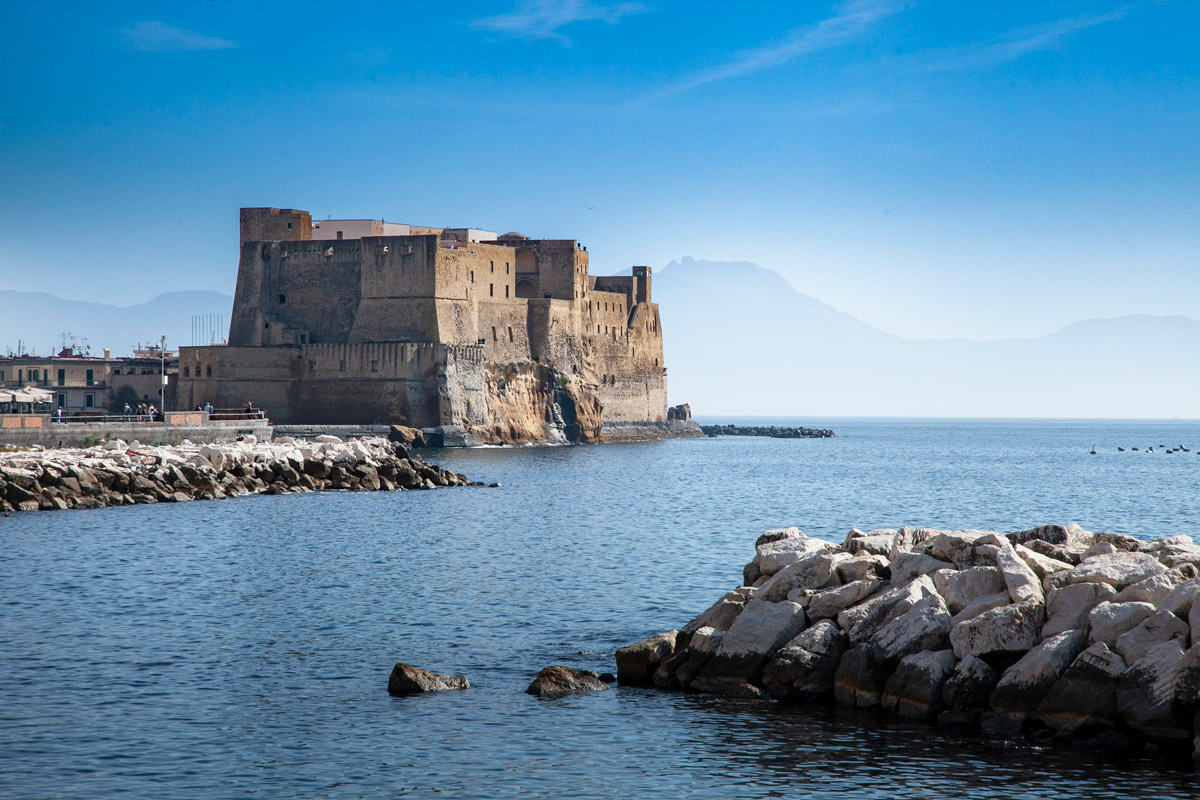
\includegraphics[width=\textwidth]{images/input_image_t5.jpg}
        \caption{(a) Input image.}
        \label{fig:test_5_input}
    \end{minipage}
    \hfill
    \begin{minipage}[b]{0.45\textwidth}
        \centering
        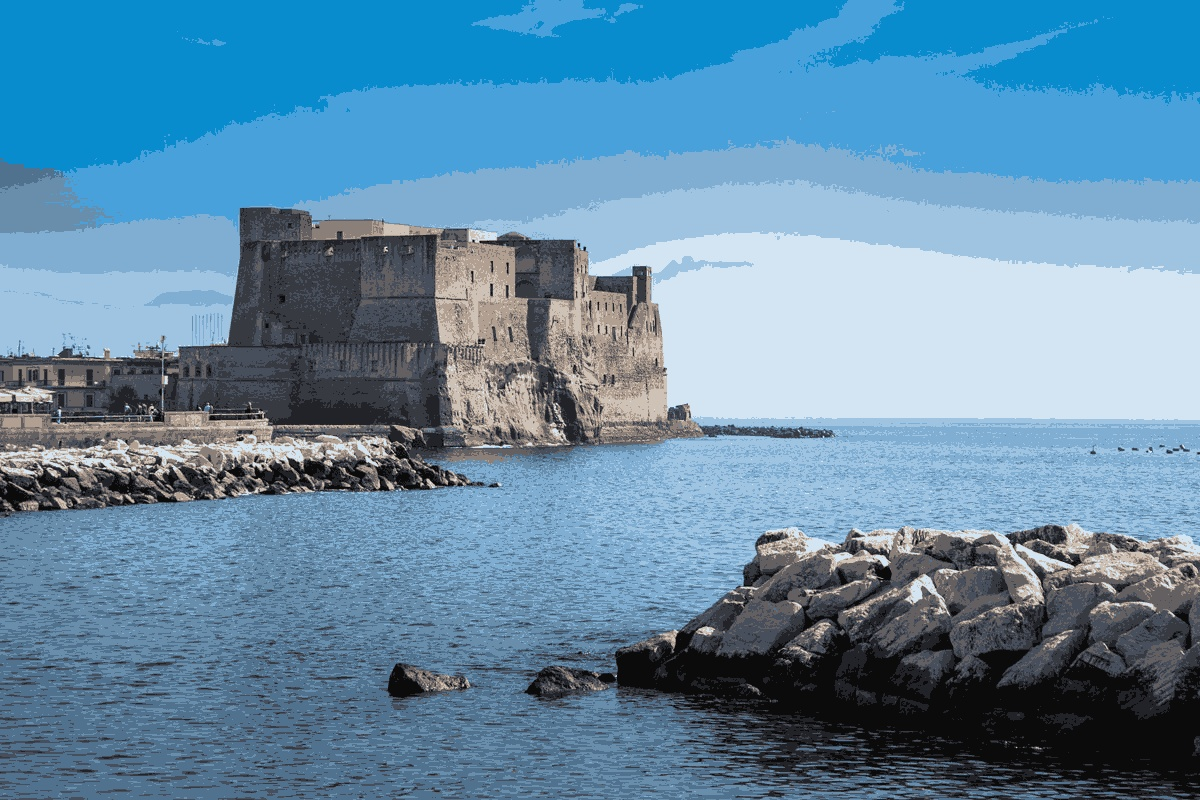
\includegraphics[width=\textwidth]{images/output_image_t5.jpg}
        \caption{(b) Output image.}
        \label{fig:test_5_output}
    \end{minipage}
    \end{figure}


    \begin{table}[H]
        \centering
        \begin{tabular}{|l|l|}
        \hline
        \textbf{Input Info}                    & \textbf{Value}                       \\ \hline
        Session ID                             & 4                                     \\ \hline
        Image width                            & 1200px                                \\ \hline
        Image height                           & 800px                                 \\ \hline
        Image channels                         & RGB (3 channels)                      \\ \hline
        \#Clusters                             & 15                                    \\ \hline
        \#Iterations                           & 100                                   \\ \hline
        \#Threads                              & 128                                   \\ \hline
        Random seed                            & 200                                   \\ \hline
        \end{tabular}
        \caption{Session information}
        \label{tab:session_information_test5}
        \end{table}
        

        \subsection{GeForce 1660}

        \begin{table}[H]
            \centering
            \begin{tabular}{|l|l|}
            \hline
            \textbf{Metric}                         & \textbf{Value}                       \\ \hline
            Execution time (Parallel version)       & ~974ms (0.9s)                        \\ \hline
            Execution time (Sequential version)     & ~4860ms (4.86s)                      \\ \hline
            Delta time                               & +3886ms (+3.88s)                     \\ \hline
            Speedup                                  & 4.9                                   \\ \hline
            \end{tabular}
            \caption{Performance Metrics on \textbf{Machine 1}}
            \label{table:performance_metrics_test5_machine1}
        \end{table}
        
        
        \subsection{Geforce 4060}
        
        \begin{table}[H]
            \centering
            \begin{tabular}{|l|l|}
            \hline
            \textbf{Metric}                         & \textbf{Value}                       \\ \hline
            Execution time (Parallel version)       & ~933ms (0.9s)                        \\ \hline
            Execution time (Sequential version)     & ~17940ms (17.9s)                     \\ \hline
            Delta time                               & +17000ms (+17s)                      \\ \hline
            Speedup                                  & 19.2                                  \\ \hline
            \end{tabular}
            \caption{Performance Metrics on \textbf{Machine 2}}
            \label{table:performance_metrics_test5_machine2}
        \end{table}
        
        
        \subsection{Quadro K5000}
        
        \begin{table}[H]
            \centering
            \begin{tabular}{|l|l|}
            \hline
            \textbf{Metric}                         & \textbf{Value}                       \\ \hline
            Execution time (Parallel version)       & ~2806ms (2.80s)                      \\ \hline
            Execution time (Sequential version)     & ~44190ms (44.19s)                    \\ \hline
            Delta time                               & +41384ms (+41.38s)                   \\ \hline
            Speedup                                  & 15.74                                 \\ \hline
            \end{tabular}
            \caption{Performance Metrics on \textbf{Machine 3}}
            \label{table:performance_metrics_test5_machine3}
        \end{table}
\subsection{Conclusion}        
In Test 5, the results demonstrate significant improvements in execution times across all machines when using parallel processing. The GeForce 1660 achieved a speedup of 4.9, showing a solid performance improvement, while the Geforce 4060 outperformed the other GPUs with a remarkable speedup of 19.2. The Quadro K5000 also demonstrated a strong performance with a speedup of 15.74, illustrating the effectiveness of parallel computation for reducing processing times.

The varying speedups suggest that the Geforce 4060 is the most efficient for this task, highlighting the benefits of modern GPUs with more computational power. The results further emphasize the importance of parallel processing in accelerating image processing tasks, particularly when working with larger datasets or more iterations. This test reinforces the continued need for optimization, as well as the value of selecting the appropriate hardware to maximize computational efficiency.

\section{Test 6}
\begin{figure}[H]
    \centering
    \begin{minipage}[b]{0.45\textwidth}
        \centering
        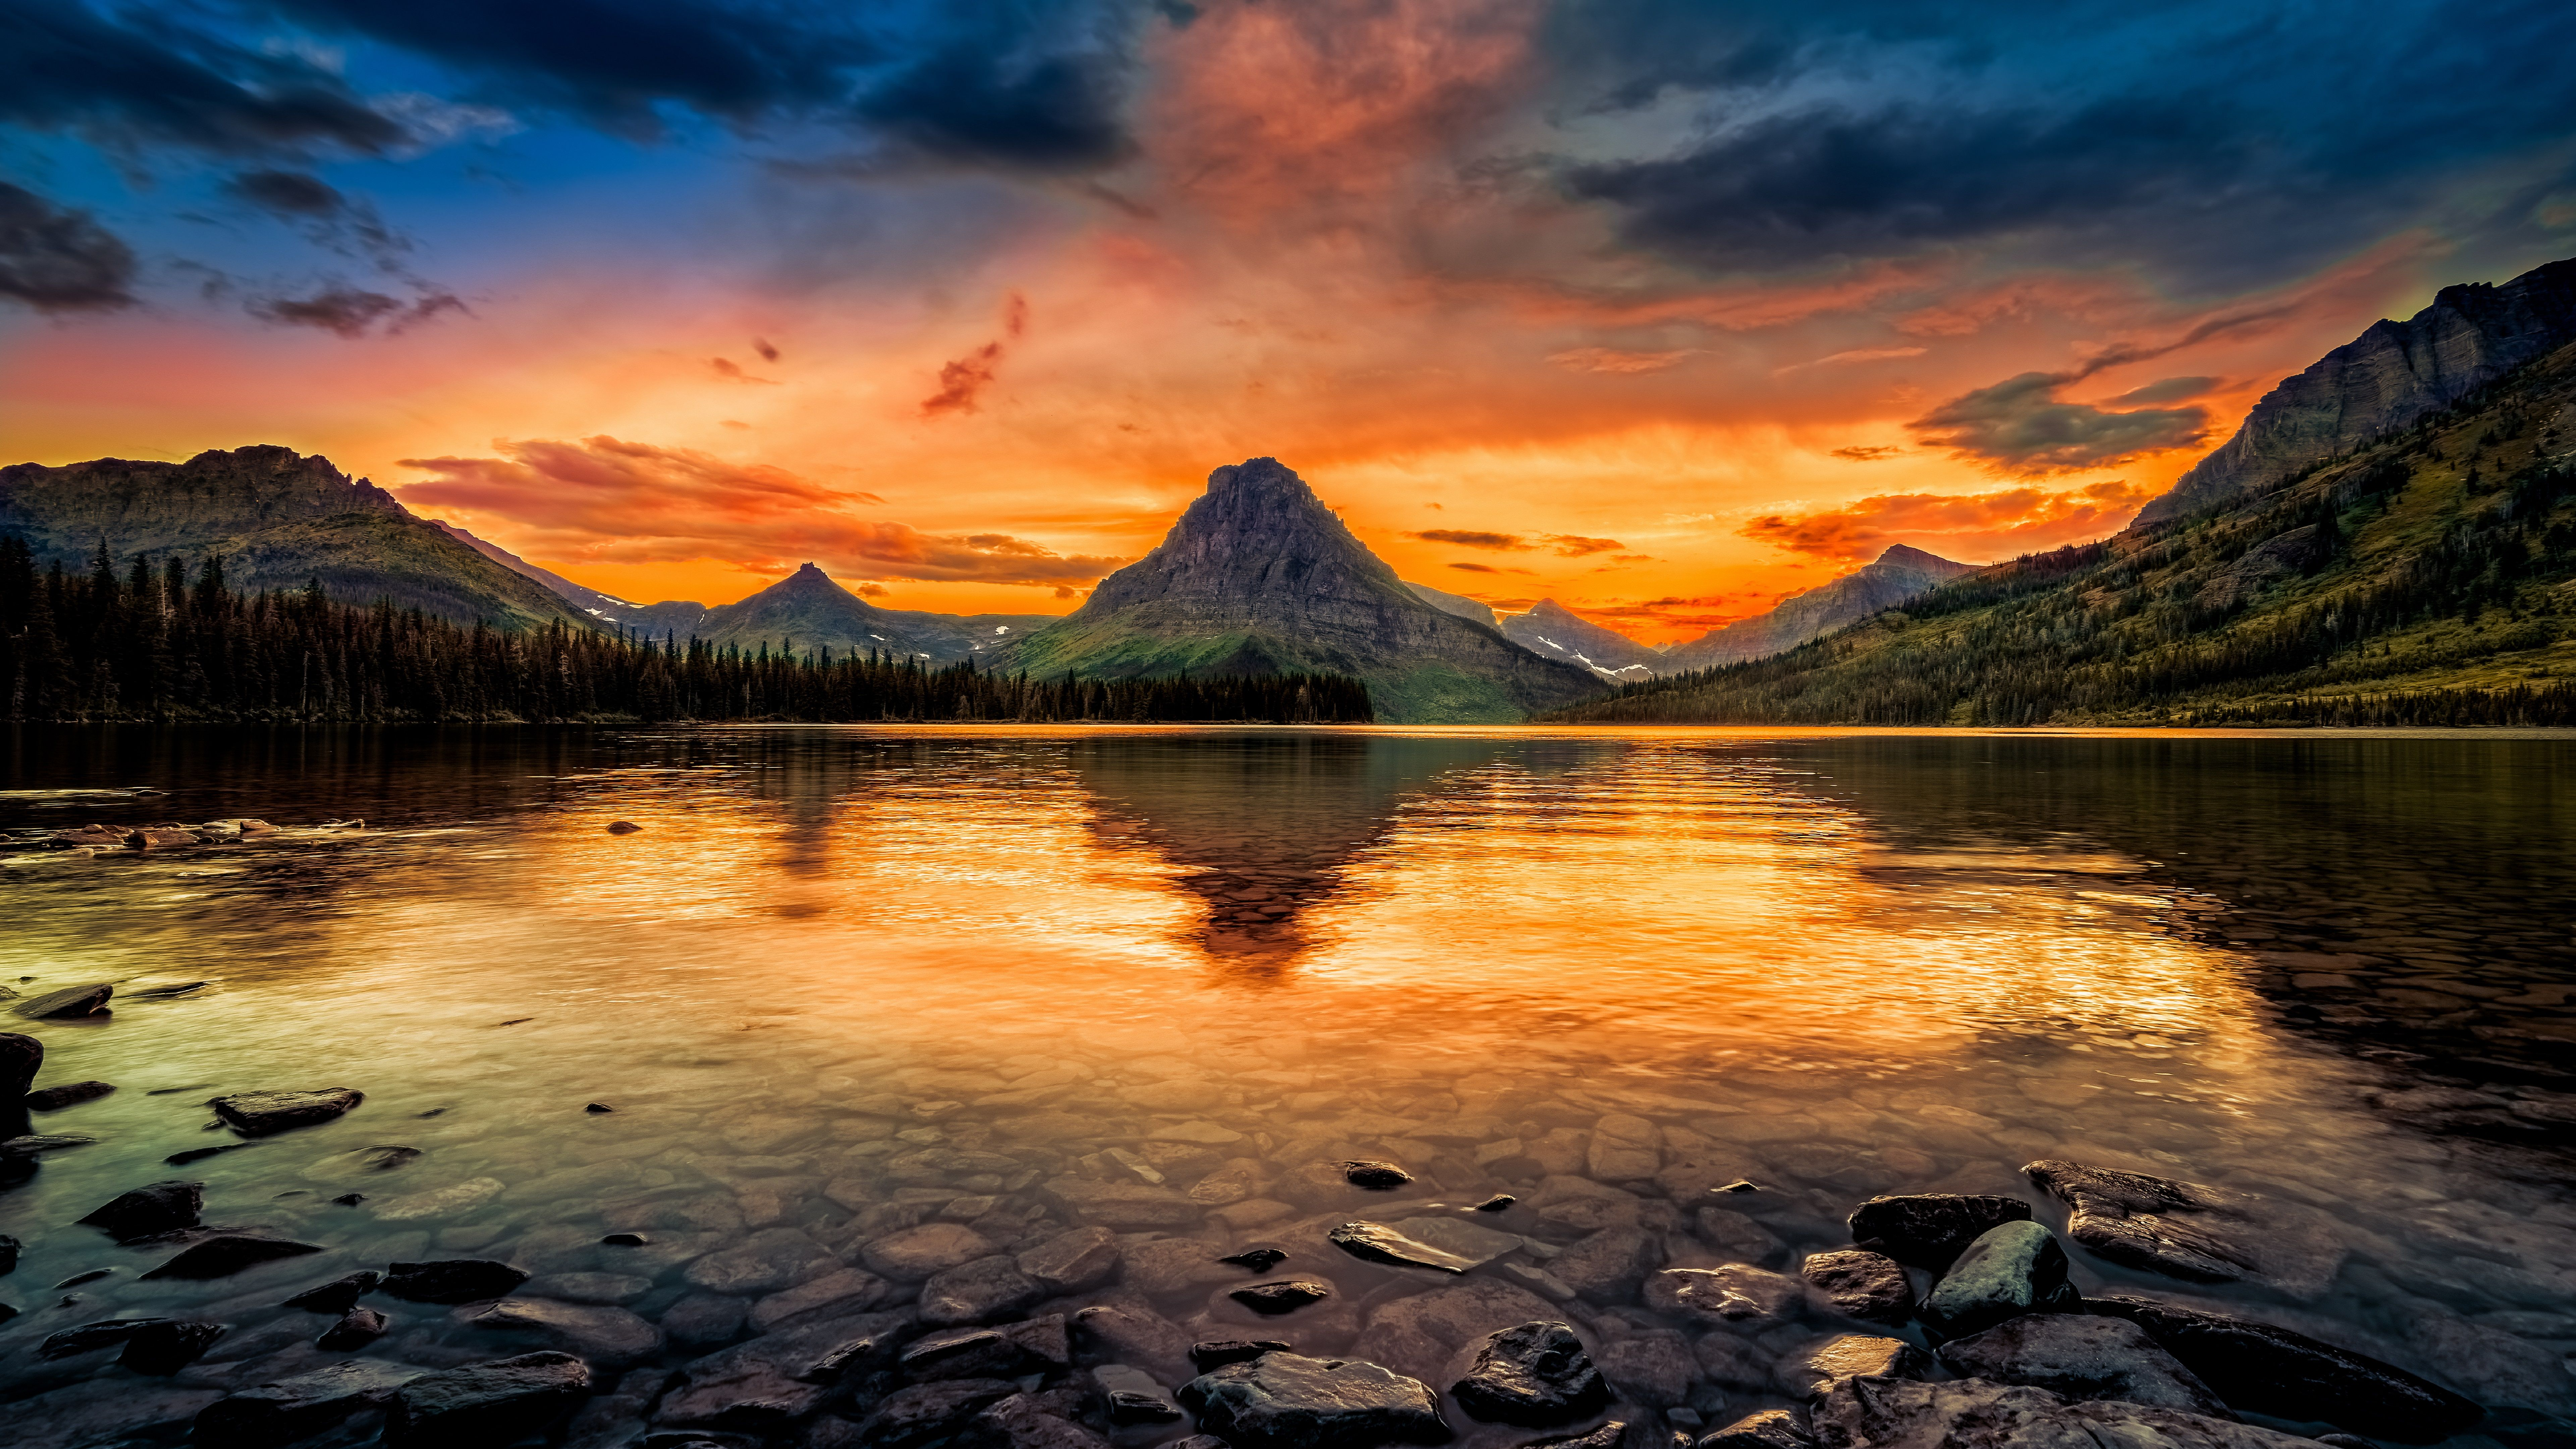
\includegraphics[width=\textwidth]{images/input_image_t6.jpg}
        \caption{(a) Input image.}
        \label{fig:test_6_input}
    \end{minipage}
    \hfill
    \begin{minipage}[b]{0.45\textwidth}
        \centering
        \includegraphics[width=\textwidth]{images/output_image_t6.jpg}
        \caption{(b) Output image.}
        \label{fig:test_6_output}
    \end{minipage}
    \end{figure}

    \begin{table}[H]
        \centering
        \begin{tabular}{|l|l|}
        \hline
        \textbf{Input Info}                    & \textbf{Value}                       \\ \hline
        Session ID                             & 5                                     \\ \hline
        Image width                            & 7680px                                \\ \hline
        Image height                           & 4320px                                \\ \hline
        Image channels                         & RGB (3 channels)                      \\ \hline
        \#Clusters                             & 15                                    \\ \hline
        \#Iterations                           & 100                                   \\ \hline
        \#Threads                              & 128                                   \\ \hline
        Random seed                            & 200                                   \\ \hline
        \end{tabular}
        \caption{Session information}
        \label{tab:session_information_test6}
        \end{table}
        

        \subsection{GeForce 1660}

        \begin{table}[H]
            \centering
            \begin{tabular}{|l|l|}
            \hline
            \textbf{Metric}                         & \textbf{Value}                       \\ \hline
            Execution time (Parallel version)       & ~39678ms (38.93s)                    \\ \hline
            Execution time (Sequential version)     & ~163920ms (2.73 minutes)             \\ \hline
            Delta time                               & +124242ms (+2.07 minutes)           \\ \hline
            Speedup                                  & 4.13                                  \\ \hline
            \end{tabular}
            \caption{Performance Metrics on \textbf{Machine 1}}
            \label{table:performance_metrics_test6_machine1}
        \end{table}
        
        
        \subsection{Geforce 4060}
        
        \begin{table}[H]
            \centering
            \begin{tabular}{|l|l|}
            \hline
            \textbf{Metric}                         & \textbf{Value}                       \\ \hline
            Execution time (Parallel version)       & ~39678ms (39.6s)                     \\ \hline
            Execution time (Sequential version)     & ~630806ms (10.5 minutes)             \\ \hline
            Delta time                               & +591128ms (+9.8 minutes)             \\ \hline
            Speedup                                  & 15.89                                 \\ \hline
            \end{tabular}
            \caption{Performance Metrics on \textbf{Machine 2}}
            \label{table:performance_metrics_test6_machine2}
        \end{table}
        
        
        \subsection{Quadro K5000}
        
        \begin{table}[H]
            \centering
            \begin{tabular}{|l|l|}
            \hline
            \textbf{Metric}                         & \textbf{Value}                       \\ \hline
            Execution time (Parallel version)       & ~100197ms (1.66 minutes)             \\ \hline
            Execution time (Sequential version)     & ~1481520ms (24.69 minutes)           \\ \hline
            Delta time                               & +1381323ms (+23.02 minutes)          \\ \hline
            Speedup                                  & 14.78                                 \\ \hline
            \end{tabular}
            \caption{Performance Metrics on \textbf{Machine 3}}
            \label{table:performance_metrics_test6_machine3}
        \end{table} 
\subsection{Conclusion}
Test 6 highlights the substantial performance improvements achieved through parallel processing. The GeForce 1660 demonstrated a speedup of 4.13, reflecting moderate acceleration, while the Geforce 4060 and Quadro K5000 showed much stronger improvements, with speedups of 15.89 and 14.78, respectively. This indicates that the more powerful GPUs, particularly the Geforce 4060, offer the most significant performance gains, reducing execution times dramatically.
The results reinforce the value of parallelization for processing large image datasets, as demonstrated by the substantial reductions in execution time when using parallel versions over sequential ones. This test further emphasizes the importance of selecting high-performance GPUs to achieve optimal efficiency for complex image processing tasks, particularly with larger images or higher iterations.        

\newpage
\section{GPUs comparison}
In this section, we present a comparison of the performance across different GPU models (GeForce 1660, GeForce 4060, and Quadro K5000) based on the execution times and overall efficiency during the various test sessions.

Figure \ref{figure:execution_time_per_session} shows the execution times for each machine across the different test sessions. From the graph, it is evident that the GeForce 4060 consistently performs faster than both the GeForce 1660 and the Quadro K5000, with the largest differences observed in the more demanding sessions (those with larger image sizes or higher iteration counts). The GeForce 1660, while generally slower, still delivers improved performance compared to the sequential version.

\begin{figure}[H]
    \centering
    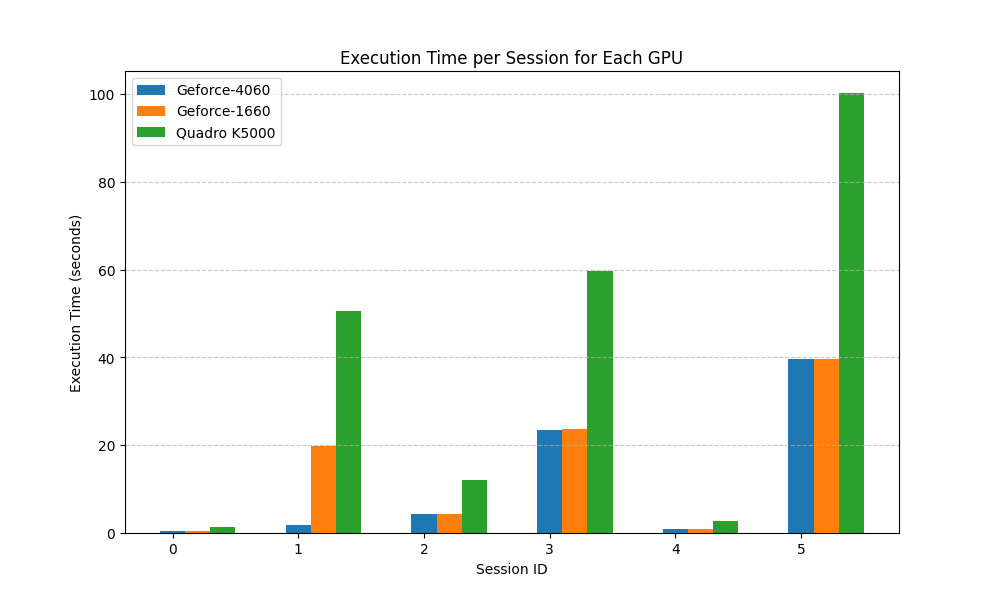
\includegraphics[width=0.8\textwidth]{images/execution_time_per_session.jpeg}
    \caption{Execution time of different machines per session}
    \label{figure:execution_time_per_session}
\end{figure}

Figure \ref{figure:execution_time_distribution} illustrates the distribution of the total execution time for each machine. This chart provides further insights into the variance in performance across the different sessions. We can observe that while the GeForce 4060 maintains a more consistent and lower execution time, the Quadro K5000 shows a larger variation in its performance across the sessions, indicating that its speedup might be more dependent on the specific task or workload.
\begin{figure}[H]
    \centering
    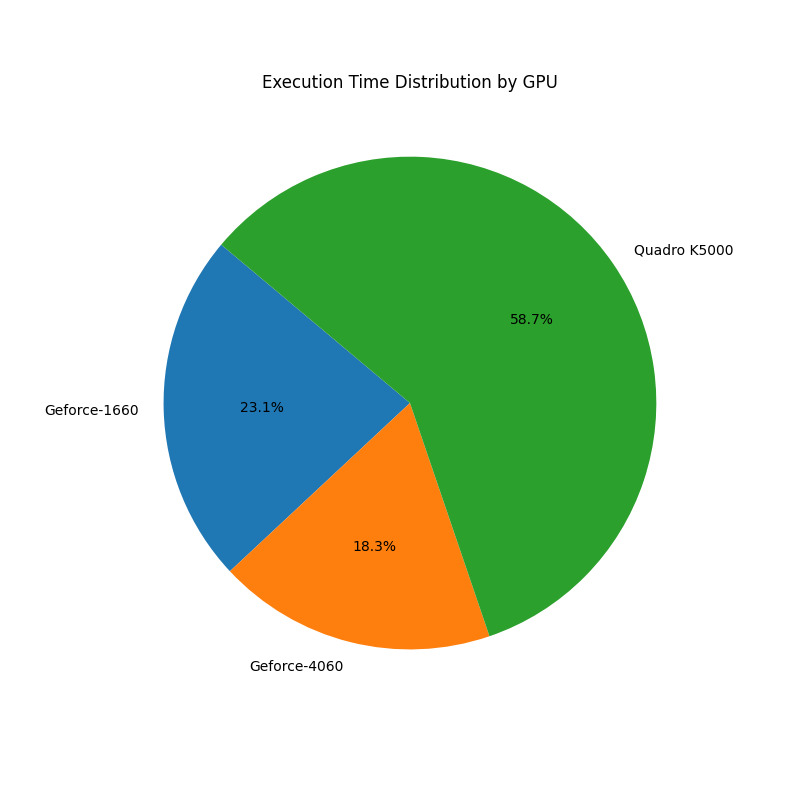
\includegraphics[width=0.6\textwidth]{images/execution_time_distribution.jpeg}
    \caption{Total execution time distribution}
    \label{figure:execution_time_distribution}
\end{figure}

Figure \ref{figure:average_gpu_time} compares the average GPU time spent processing tasks across all sessions for each GPU. As expected, the GeForce 4060 exhibits the lowest average GPU time, followed by the GeForce 1660 and Quadro K5000. This result highlights the efficiency of the newer, more powerful GeForce 4060 in handling image processing tasks and emphasizes the role of GPU architecture in optimizing computational workloads.
\begin{figure}[H]
    \centering
    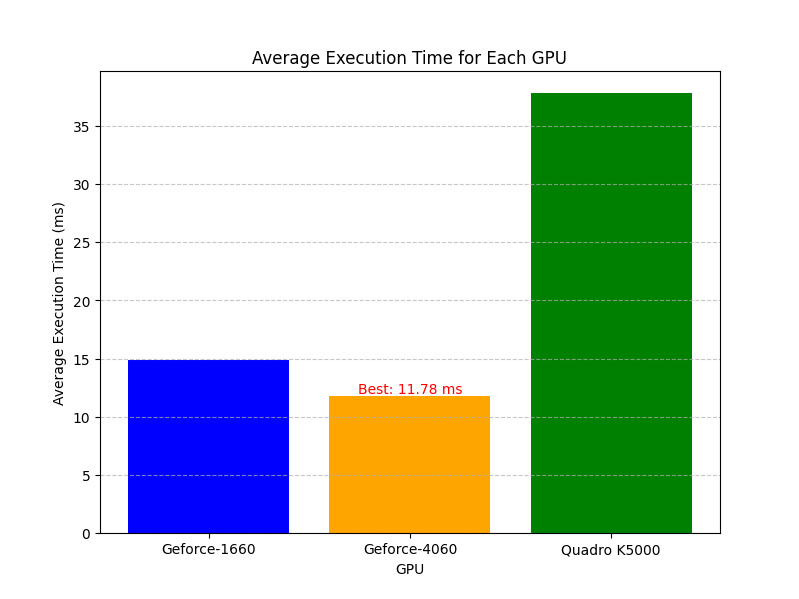
\includegraphics[width=0.6\textwidth]{images/average_gpu_time.jpeg}
    \caption{Average GPU time comparison}
    \label{figure:average_gpu_time}
\end{figure}

\section{Discussion}
We evaluated the performance of various GPU models (GeForce 1660, GeForce 4060, and Quadro K5000) across several test scenarios, analyzing the effectiveness of parallel processing for image-based tasks. The results clearly demonstrate the significant advantages of using parallel processing over sequential approaches, with notable speedup improvements observed across all GPU models.
Key findings include:
\begin{itemize}
    \item The GeForce 4060 consistently outperformed the other GPUs, delivering the highest speedup and reducing execution times substantially, especially with larger image sizes and higher iteration counts.
    \item The Quadro K5000, while slower than the GeForce 4060, still demonstrated a solid performance improvement over the sequential version, making it a strong option for large-scale image processing tasks.
    \item The GeForce 1660, although providing modest speedups, was still able to achieve faster execution times than the sequential version, highlighting the benefit of parallelization even with mid-range GPUs.
\end{itemize}

These results underscore the importance of parallel computing for image processing tasks, where GPU acceleration plays a pivotal role in reducing computation time and enabling real-time or near-real-time processing. The choice of GPU significantly impacts performance, with high-end models like the GeForce 4060 providing the most noticeable improvements.


\printbibliography
\end{document}  % Fine del documento